\documentclass[a4paper]{article}

\usepackage{pdp}
\usepackage{float}
\usepackage{listings}
\usepackage{xcolor}
\usepackage{tikz}
\usepackage{amssymb}
\usetikzlibrary{positioning, shapes, arrows.meta}
\usepackage{hyperref}
\usepackage{tabularx}
\usepackage{makecell}
\usepackage{amsmath}
%------------------------------------------------------------------------------
% Configuration de l'environnement de code (lstlisting)
%------------------------------------------------------------------------------
\definecolor{codegray}{rgb}{0.5,0.5,0.5}
\definecolor{codeblue}{rgb}{0.0,0.0,0.6}
\definecolor{codegreen}{rgb}{0.0,0.5,0.0}
\definecolor{codebg}{rgb}{0.97,0.97,0.97}

\lstdefinestyle{cstyle}{
    language=C,
    backgroundcolor=\color{codebg},
    basicstyle=\ttfamily\footnotesize,
    keywordstyle=\color{codeblue}\bfseries,
    commentstyle=\color{codegreen}\itshape,
    stringstyle=\color{red!70!black},
    numberstyle=\tiny\color{codegray},
    numbers=left,
    numbersep=8pt,
    stepnumber=1,
    frame=single,
    framesep=4pt,
    rulecolor=\color{codegray!40},
    breaklines=true,
    breakatwhitespace=true,
    captionpos=b,
    tabsize=2,
    showstringspaces=false,
    morekeywords={bool, size_t, ssize_t, tcp_buffer_t, NetworkManager,
                  Packet, PacketType, ServerContext, ClientContext,
                  NetworkEvents, ConnectedClient, ClientStatus,
                  GameState, Move, time_t, AppContext, GtkWidget,
                  GtkApplication, GtkStack, GuiPhase, KeyBindings}
}
\lstset{style=cstyle}

%------------------------------------------------------------------------------
%	REPORT INFORMATION
%------------------------------------------------------------------------------

\title{Jeu des Amazones -- Projet C}
\subtitle{Rapport final}
\author{Nicolas Caminade, Etudiant2, Etudiant3, Etudiant4, Etudiant5}

%------------------------------------------------------------------------------

\begin{document}

%------------------------------------------------------------------------------
%	TITLE PAGE
%------------------------------------------------------------------------------

\maketitle
\thispagestyle{empty}



%------------------------------------------------------------------------------
%	MAIN MATTER
%------------------------------------------------------------------------------

\section{Introduction}

Le jeu des Amazones est un jeu de société combinatoire abstrait inventé
par l'Argentin Walter Zamkauskas en 1988 et publié pour la première fois
dans la revue \textit{El Acertijo} en 1992~\cite{zamkauskas1992}. Il se joue
traditionnellement sur un plateau de 10$\times$10 cases et combine des
éléments des échecs (le déplacement de la dame) et du jeu de Go (le contrôle
du territoire).

\subsection{Historique}

Né en Argentine dans les années 1980, le Jeu des Amazones a d'abord circulé
dans des cercles restreints d'amateurs de jeux abstraits avant d'être diffusé
internationalement par la revue \textit{El Acertijo} en 1992. Sa popularité
auprès de la communauté informatique ne tardera pas à se manifester~: dès la
fin des années 1990, des chercheurs en intelligence artificielle s'emparent du
jeu comme banc d'essai pour les algorithmes de recherche arborescente.

En 2005, l'équipe de Furtak démontre mathématiquement que résoudre ce jeu de
manière générale est un problème PSPACE-complet~\cite{furtak2005generalized},
une classe de difficulté supérieure aux problèmes NP classiques, ce qui
confirme définitivement que le jeu résiste à toute résolution exhaustive.
Richard Lorentz établit ensuite, avec son programme \textit{Invader}, que
l'approche statistique du Monte Carlo Tree Search (MCTS) constitue à ce jour
la stratégie la plus performante face à l'explosion combinatoire
propre au jeu~\cite{lorentz2008amazons}. Depuis lors, des chercheurs
intègrent des techniques de \textit{Deep Learning} et de réseaux de
neurones pour tenter de dépasser cet algorithme~\cite{9534274}.

\subsection{Règles}

Le Jeu des Amazones se pratique sur un damier, traditionnellement de
$10 \times 10$ cases. Chaque joueur dispose de quatre amazones, disposées
symétriquement en début de partie selon une configuration initiale précise~:
les Blancs placent leurs pièces en (d1), (g1), (a4) et (j4), tandis que les
Noirs occupent les cases (d10), (g10), (a7) et (j7). Cette disposition
garantit un équilibre stratégique parfait entre les deux camps.

\paragraph{Objectif du jeu.}
La victoire revient au dernier joueur capable d'effectuer un coup légal.
L'enjeu est donc de priver progressivement l'adversaire de tout espace de
déplacement en combinant occupation du terrain et tirs de flèches. Contrairement
aux jeux comme les échecs ou le Go, il n'existe pas de capture de pièce~: le
matériel reste constant tout au long de la partie.

\paragraph{Déroulement d'un tour.}
Chaque tour est impérativement composé de deux phases successives et
indissociables. Dans un premier temps, le joueur choisit l'une de ses
amazones et la déplace en ligne droite --- verticalement, horizontalement ou
en diagonale --- vers une case libre. Ce mouvement est identique à celui de
la dame aux échecs~: l'amazone peut parcourir autant de cases qu'elle le
souhaite dans la direction choisie, mais elle ne peut ni traverser ni
s'arrêter sur une case occupée par une autre pièce (amie ou ennemie) ou par
une flèche. Dans un second temps, depuis sa nouvelle position, cette même
amazone doit obligatoirement tirer une flèche. La flèche obéit aux mêmes
règles de trajectoire que l'amazone~: elle se déplace en ligne droite dans
l'une des huit directions possibles, sans pouvoir franchir d'obstacle. La
case où la flèche atterrit est définitivement brûlée et inaccessible pour le
reste de la partie.

\paragraph{Subtilités tactiques.}
Une règle souvent mal comprise par les débutants concerne le tir de la
flèche~: l'amazone peut tirer dans n'importe quelle direction autorisée
depuis sa case d'arrivée, y compris en direction de la case qu'elle vient
de quitter. Cette subtilité ouvre des possibilités tactiques riches, notamment
la possibilité de s'auto-bloquer temporairement pour mieux circonscrire
l'adversaire. De plus, la flèche ne peut traverser une case occupée par
une amazone adverse, ce qui signifie que les pièces ennemies servent
d'obstacles naturels aux tirs.

\paragraph{Fin de partie et variantes.}
Le jeu des Amazones ne connaît pas de match nul par répétition ou par
épuisement de matériel~: puisque chaque tour réduit irrémédiablement le
nombre de cases disponibles, la partie se termine forcément par le blocage
complet d'un joueur. En pratique, les parties se divisent souvent en deux
phases distinctes~: une ouverture stratégique où les amazones s'affrontent
pour le contrôle des grandes zones du plateau, suivie d'une phase finale
où chaque joueur maximise son territoire cloisonné. Bien que le format
$10 \times 10$ soit le standard, des variantes sur plateau $6 \times 6$ ou
$8 \times 8$ existent avec un nombre d'amazones adapté, permettant des parties
plus rapides tout en conservant la richesse tactique du jeu.

\begin{figure}[ht]
\centering
%\includegraphics[width=0.22\textwidth]{defaultStateboard.png}
%\includegraphics[width=0.22\textwidth]{1wallplacedboard.png}
\caption{Évolution d'une partie~: position initiale et premier
coup~\cite{img0}\cite{img1}}
\end{figure}

\subsection{Complexité} \label{sec:complexite}

Le jeu des Amazones est d'une très grande complexité~\cite{Complexite}.
Le tableau ci-dessous emploie les abréviations Branch.~pour «~facteur de
branchement~» et Cmplx.~pour «~complexité~».

\begin{table}[H]
    \centering
\renewcommand{\arraystretch}{1.5}
\resizebox{\textwidth}{!}{
\begin{tabular}{ | p{4.5cm} || c | c | c | }
    \hline
    \textbf{} & \textbf{Échecs} & \textbf{Amazones} & \textbf{Go} \\
    \hline
    Facteur Branch. Initial
    & $\mathtt{\sim}$ 20
    & \makecell{$\mathtt{\sim}$ 2176}
    & $\mathtt{\sim}$ 361 \\
    \hline
    Facteur Branch. Moyen
    & $\mathtt{\sim}$ 35
    & \makecell{$\mathtt{\sim}$ 374 joueur de départ \\ $\mathtt{\sim}$ 299 deuxième joueur \\ $\mathtt{\sim}$50 durant la fin de partie}
    & $\mathtt{\sim}$ 250 \\
    \hline
    Nombre de tours moyen
    & $\mathtt{\sim}$ 80
    & $\mathtt{\sim}$ 84
    & $\mathtt{\sim}$ 150 \\
    \hline
    Cmplx. Arbre de jeu
    & $\mathtt{\sim} 10^{123}$
    & $\mathtt{\sim}$ 1.09 * $10^{212}$
    & $\mathtt{\sim} 10^{360}$ \\
    \hline
    Cmplx. Espaces d'états
    & \makecell{de $\mathtt{\sim}$ 3.7 * $10^{43}$ à $\mathtt{\sim}$ $10^{52}$}
    & $\mathtt{\sim}$ 6.45* $10^{40}$
    & $\mathtt{\sim}$ $10^{170}$ \\
    \hline
\end{tabular}
}
\caption{Comparaison des complexités pour un plateau traditionnel (8$\times$8
pour les échecs, 10$\times$10 pour les Amazones, 19$\times$19 pour le Go)
\cite{complexities}\cite{gocomplexity}}
\end{table}
\renewcommand{\arraystretch}{1}

Comme l'illustre ce tableau comparatif, la complexité des Amazones réside
dans son facteur de branchement initial extrême, surpassant largement celui
des échecs et comparable à celui du Go. Bien que la profondeur de jeu soit
modérée, cette «~largeur~» excessive génère un arbre de jeu colossal
($10^{212}$), rendant toute exploration exhaustive impossible en raison de
l'explosion combinatoire. Pour contourner cette explosion, les approches
modernes s'appuient sur la sélectivité~: solveurs de preuve comme
\textit{df-pn}~\cite{dfpn}, algorithmes de jeu utilisant du
\textit{Forward Pruning}~\cite{fpruning}, méthodes statistiques comme le MCTS
via l'Upper Confidence bounds applied to Trees (UCT)~\cite{uct}, ou encore
le Machine Learning.


\section{Algorithmes et structures de données}

\subsection{Le cœur du jeu et l'Intelligence Artificielle}
\label{sec:ai-alg-struct}

\subsubsection{Représentation de l'état~: les Bitboards}

Pour garantir des performances optimales, nous avons modélisé le plateau
via des \textit{Bitboards} \cite{Browne2014}. Le plateau pouvant atteindre une taille de
11$\times$11 (121 cases), une simple variable de 64 bits était insuffisante.
Nous avons donc conçu une structure \texttt{Bitboard} composée de deux
entiers non signés ($2 \times$\texttt{uint64\_t}), offrant 128 bits
d'espace.

Cette structure permet de valider des coups ou de calculer des territoires
en temps constant $\mathcal{O}(1)$ via des opérations bit-à-bit~: ET, OU,
XOR, décalages, \textit{Pop Least-Significant-Bit}. La véritable puissance
de cette structure s'exprime lors de la génération des trajectoires
(\textit{slides}). Dans nos heuristiques, nous distinguons deux types
d'expansions~: le \textbf{\textit{King step}}, qui simule une avancée d'une
seule case dans les huit directions, et le \textbf{\textit{Queen slide}},
qui calcule la portée maximale d'une pièce sur ses lignes, colonnes et
diagonales avant de rencontrer un obstacle.

Pour calculer ces \textit{Queen slides} sans boucles itératives
conditionnelles coûteuses, nous avons implémenté l'algorithme de
\textbf{Kogge-Stone} \cite{CPW_KoggeStone}. Issu de l'architecture des additionneurs matériels,
cet algorithme utilise le principe de propagation parallèle
(\textit{Parallel Prefix})~: il «~pousse~» simultanément tous les bits
représentant nos pièces à travers un masque de cases vides, en utilisant
des décalages bit-à-bit successifs et exponentiels (1, puis 2, puis 4,
puis 8). L'intégralité des trajectoires possibles dans une direction donnée
est ainsi calculée en seulement quatre instructions, couvrant largement la
distance maximale de onze cases.

\subsubsection{Analyse de Complexité des Opérations Bitboards}

La majeur partie de nos opérations fondamentales sur les \textit{Bitboards} s'exécutent en temps constant $\mathcal{O}(1)$. Il convient cependant de distinguer la complexité unitaire des instructions matérielles de leur application algorithmique :

\begin{itemize}
    \item \textbf{Opérations basiques en $\mathcal{O}(1)$ :} Les manipulations de masques (ET, OU, XOR) ainsi que les décalages de bits s'exécutent en un nombre fixe de cycles d'horloge. Le calcul du débordement entre nos deux entiers 64 bits (\texttt{low} et \texttt{high}) ajoute un surcoût mineur de quelques instructions processeur, mais la complexité temporelle globale reste strictement bornée et totalement indépendante de l'état du plateau.
    
    \item \textbf{Expansions spatiales en $\mathcal{O}(1)$ :} C'est sur ce point que l'architecture Bitboard surpasse drastiquement les approches matricielles. La génération des trajectoires (\textit{slides}), qu'il s'agisse d'un pas de Roi ou du calcul de la portée maximale d'une Reine, s'effectue en temps constant global. Notre implémentation de l'algorithme de Kogge-Stone déroule en effet une séquence stricte de 4 opérations de décalages exponentiels (1, 2, 4, 8) bornés par des masques. Le processeur calcule ainsi l'expansion de \textit{toutes} les pièces de la même couleur de manière parfaitement simultanée, sans avoir recours à la moindre boucle conditionnelle.
    
    \item \textbf{Extraction et itération conditionnelle en $\mathcal{O}(k)$ :} La seule véritable complexité variable de notre modèle intervient lors de la sérialisation des coups ou de l'évaluation des heuristiques. La fonction unitaire d'extraction \texttt{pop\_lsb} s'exécute instantanément en $\mathcal{O}(1)$ grâce à un appel d'instruction matérielle spécifique. Toutefois, cette fonction est invoquée au sein d'une boucle. Cette boucle s'exécute donc exactement $k$ fois, où $k$ est le nombre strict de pièces actives évaluées. Nous garantissons ainsi une complexité algorithmique d'itération en $\mathcal{O}(k)$, un comportement infiniment plus performant qu'un parcours complet de la grille en $\mathcal{O}(N)$ inhérent aux tableaux bidimensionnels classiques.
\end{itemize}

\subsubsection{L'approche Minimax et ses heuristiques}

Le premier moteur d'IA repose sur l'algorithme Minimax, optimisé par
l'élagage Alpha-Beta \cite{GeeksforGeeks2026_AlphaBeta}. Pour pallier l'explosion combinatoire, nous avons
enrichi cette base par deux mécanismes paramétrables. L'approfondissement
itératif (\textit{Iterative Deepening}) garantit le renvoi du meilleur coup
trouvé à la profondeur maximale complétée si la limite de temps est atteinte.
L'élagage anticipé (\textit{Forward Pruning} \cite{Qian2015}) restreint la largeur du
faisceau de recherche en ne conservant que les coups offrant le plus de
mobilité. Sans ces optimisations, le système bascule de manière transparente
sur un Alpha-Beta exhaustif classique.

L'évaluation des nœuds feuilles constitue le cœur décisionnel de notre
stratégie. Nous avons conçu et comparé trois fonctions d'évaluation offrant
un compromis graduel entre rapidité et finesse mathématique.

La première approche est l'évaluation de mobilité \cite{Hensgens2001}, axée sur la mobilité relative (\texttt{eval\_me}),
calcule rapidement la différence entre le nombre total de coups légaux
disponibles pour les Blancs et les Noirs. En simulant une expansion de type
\textit{Queen slide} pour toutes les reines, l'algorithme dénombre les cases
uniques atteignables. Soit $M_p$ l'ensemble des cases atteignables par le
joueur $p$, l'heuristique est définie par~:
$$ \mathcal{H}_{me} = |M_{blanc}| - |M_{noir}| $$
Cette légèreté calculatoire permet d'atteindre d'excellentes profondeurs
d'exploration, mais l'évaluation demeure myope et peine à anticiper la
fermeture structurelle des territoires.

La deuxième heuristique, dite de territoire relatif (\texttt{eval\_rth}) \cite{Hensgens2001},
évalue le contrôle spatial en déployant un parcours en largeur (BFS)
simultané. Elle calcule la distance, en nombre de mouvements de Reine,
séparant chaque case vide de la pièce la plus proche. Soit $\mathcal{E}$
l'ensemble des cases vides, et $d_W(x)$ (resp. $d_B(x)$) la distance minimale
entre une case $x$ et une reine blanche (resp. noire)~:
$$ \mathcal{H}_{rth} = \sum_{x \in \mathcal{E}} \Delta(x) \quad \text{avec} \quad \Delta(x) =
\begin{cases}
\min(d_B(x), C) - d_W(x) & \text{si } d_W(x) < d_B(x) \\
-(\min(d_W(x), C) - d_B(x)) & \text{si } d_B(x) < d_W(x) \\
0 & \text{sinon}
\end{cases} $$
Une distance infinie est plafonnée par une constante $C$ (définie par
$C = \text{taille du plateau} + 2$).

Notre modèle le plus abouti repose sur les territoires absolus combinés
(\texttt{eval\_qdkd}) \cite{Lieberum2005}. Il simule l'appropriation du plateau par une
expansion continue (\textit{flood-fill}) traitée case par case. La force
de cette heuristique réside dans sa résolution des conflits~: si une case
est atteinte par les deux joueurs à la même itération $k$, elle est déclarée
contestée et agit comme un obstacle infranchissable. Soient $T_Q(p)$ et
$T_K(p)$ les ensembles de cases conquises par le joueur $p$ selon des
déplacements respectifs de Reine et de Roi~:
$$ t_1 = |T_Q(Blanc)| - |T_Q(Noir)| \qquad t_2 = |T_K(Blanc)| - |T_K(Noir)| $$
Le calcul final applique une pondération mariant vision globale et contrôle
local~ (choisi d'après les pistes de calcul de Lieberum \cite{Lieberum2005}) :
$$ \mathcal{H}_{qdkd} = 1.0 \times t_1 + 0.5 \times t_2 $$

\subsubsection{Monte Carlo Tree Search (MCTS) et apprentissage automatique}

Le second moteur d'IA exploite le Monte Carlo Tree Search. Pour modéliser
l'arborescence, nous avons opté pour une structure de données
\textbf{LCRS} (\textit{Left-Child Right-Sibling}) \cite{GeeksforGeeks2025_LCRS}. Ce choix découle
directement du facteur de branchement initial supérieur à 2\,000 coups
possibles~: utiliser des tableaux de pointeurs pour stocker les enfants
de chaque nœud aurait provoqué une explosion de l'empreinte mémoire.
Le choix de la structure LCRS (\textit{Left-Child Right-Sibling}) répond à une contrainte majeure du jeu des Amazones~: son facteur de branchement exceptionnellement élevé (entre 500 et 2\,000 coups possibles par tour). Une approche classique, où chaque nœud pré-allouerait un tableau pointant vers tous ses enfants potentiels, saturerait la mémoire système de manière quasi instantanée. 

À l'inverse, l'approche LCRS garantit une empreinte mémoire minimale et fixe. Chaque nœud ne contient que deux pointeurs~: l'un vers son premier enfant, l'autre vers son frère immédiat. Cette optimisation spatiale implique un compromis temporel, car l'accès au $k$-ième enfant nécessite un parcours séquentiel en $O(k)$ cycles CPU. 

Cependant, ce coût est largement justifié. Couplée à une instanciation dynamique des enfants --- où un nœud n'est créé que lorsque le coup correspondant est réellement exploré --- cette architecture empêche l'explosion mémoire tout en garantissant l'efficacité du moteur.
Nous avons également enrichi ce MCTS d'un réseau de neurones. Dans ce mode,
l'évaluation des nœuds non terminaux est combinée à l'inférence d'un modèle 
TensorFlow recevant en entrée un tenseur à quatre canaux généré par nos bitboards.

\paragraph{Politique de sélection UCT standard.}
Dans sa version classique, le MCTS guide la phase de sélection de l'arborescence à l'aide de la formule \textbf{UCT} (\textit{Upper Confidence bounds applied to Trees}) \cite{Kocsis2006}. Cette métrique applique les principes des bandits manchots à la recherche arborescente afin de trouver le compromis mathématique optimal entre l'exploitation des branches prometteuses et l'exploration des chemins peu visités. Pour un nœud enfant $n$, l'évaluation s'écrit~:

$$ \text{UCT}(n) = Q(n) + c \cdot \sqrt{\frac{\ln(N(parent))}{N(n)}} $$

où $Q(n)$ représente la valeur moyenne empirique du nœud (le taux de victoire obtenu par les simulations aléatoires), $N(parent)$ et $N(n)$ désignent respectivement le nombre total de visites du nœud parent et de l'enfant évalué, et $c$ est la constante d'exploration (théoriquement fixée à $\sqrt{2}$). Le premier terme favorise l'exploitation pure, tandis que le second garantit une exploration continue~: la racine carrée croît de manière logarithmique avec les visites du parent, forçant l'algorithme à évaluer les enfants délaissés (où $N(n)$ est faible ou nul).

\paragraph{Variante PUCT pour l'apprentissage automatique.} 
Lorsque le réseau de neurones est activé, la politique de sélection UCT classique est remplacée par la variante \textbf{PUCT} (\textit{Predictor + Upper Confidence Bound}) \cite{Cazenave2022}. Cette approche hybride combine l'exploration statistique d'UCT avec une évaluation par réseau de neurones pour guider plus efficacement la recherche.

La formule PUCT pour un nœud enfant $n$ s'écrit~:
$$ \text{PUCT}(n) = \frac{Q_{\text{rollout}}(n) + Q_{\text{NN}}(n)}{2} + c_{\text{puct}} \cdot \frac{\sqrt{N(parent)}}{1 + N(n)} $$

où $Q_{\text{rollout}}(n)$ est le taux de victoire empirique obtenu par les simulations Monte Carlo, $Q_{\text{NN}}(n)$ est la probabilité de victoire prédite par le réseau de neurones, $N(parent)$ et $N(n)$ sont respectivement les nombres de visites du parent et de l'enfant, et $c_{\text{puct}}$ est une constante d'exploration (par défaut 1.5).

Le réseau de neurones utilisé est un modèle de régression linéaire simple entraîné sur des parties auto-générées. Il reçoit en entrée un tenseur de dimension $11 \times 11 \times 4$ représentant~:
\begin{itemize}
    \item Canal 0~: positions des reines blanches (1 si présente, 0 sinon)
    \item Canal 1~: positions des reines noires
    \item Canal 2~: positions des flèches
    \item Canal 3~: masque de validité du plateau (1 pour les cases valides)
\end{itemize}

Cette architecture à quatre canaux permet au modèle de capturer simultanément la configuration matérielle et la topologie du plateau. Lors de la sélection, si l'évaluation neuronale d'un nœud n'a pas encore été calculée (\texttt{ai\_eval} $\leq -2.0$), le tenseur correspondant est généré à la volée et soumis au modèle TensorFlow. La valeur retournée est ensuite mise en cache dans le nœud pour éviter les inférences redondantes.


 
%------------------------------------------------------------------------------
% SECTION 2.2 - Structures de données et protocole réseau
%------------------------------------------------------------------------------
 
\subsection{Réseau~: structures de données et protocole}
\label{sec:network-data}
 
La mise en place du mode multijoueur a nécessité de résoudre deux contraintes
fondamentales de la programmation réseau~: la nature orientée flux du protocole
TCP et la nécessité de maintenir un état cohérent pour chaque connexion
asynchrone. Cette section présente les structures de données conçues pour
répondre à ces exigences.
 
\subsubsection{Le problème du \textit{Framing} TCP}
\label{subsec:tcp-framing}
 
Contrairement à UDP qui fonctionne par datagrammes délimités, TCP est orienté
flux~: l'émetteur peut envoyer trois messages de 100 octets, mais le récepteur
pourrait recevoir un bloc de 250 octets suivi d'un fragment de 50 octets. Ce
phénomène, appelé \textit{TCP Framing}, rend impossible la lecture directe de
messages individuels sans mécanisme de délimitation.
 
\paragraph{Choix du délimiteur.}
Nous avons opté pour un délimiteur de fin de message (\texttt{'\textbackslash{}n'})
plutôt qu'un préfixe de longueur. Ce choix s'inscrit dans la tradition des
protocoles applicatifs textuels (SMTP, POP3, IRC) et présente deux avantages~:
il permet le débogage à l'œil nu via des outils standards (\texttt{netcat},
\texttt{tcpdump}), et il évite les problèmes de désynchronisation si un octet
de longueur est corrompu --- une erreur dont la récupération serait impossible
sans fermer la connexion.
 
\paragraph{Structure de tampon.}
Pour accumuler les fragments TCP jusqu'à réception d'un message complet, chaque
connexion dispose de son propre tampon linéaire de 4\,096 octets. Ce
dimensionnement (environ 2,7 fois le MTU Ethernet standard de 1\,500 octets)
garantit qu'au moins deux messages complets peuvent être mis en file
simultanément, absorbant ainsi les pics de trafic sans saturation.
 
\paragraph{Algorithme d'extraction.}
L'extraction des messages s'effectue en trois phases distinctes. La première
phase consiste en l'\textbf{accumulation}~: les octets bruts reçus via
\texttt{recv()} sont concaténés à la fin du tampon. La deuxième phase est la
\textbf{recherche}~: une recherche linéaire localise le premier caractère
de fin de ligne dans le tampon. La troisième phase est la \textbf{consommation}~:
le message extrait est copié vers un tampon de sortie, puis les octets restants
sont décalés vers le début du tampon via \texttt{memmove()}, préservant ainsi
les fragments du message suivant. Cette dernière opération, bien que coûteuse
en temps ($\mathcal{O}(n)$ où $n$ est la taille des données restantes), reste
négligeable face aux latences réseau et garantit une gestion mémoire sans
fragmentation.
 
\subsubsection{Protocole applicatif et sérialisation}
\label{subsec:protocol}
 
Au-dessus de la couche de framing, nous avons défini un protocole applicatif
textuel structuré autour d'une unité atomique~: le \texttt{Packet}.
 
\paragraph{Choix du format texte.}
Le format ASCII a été préféré au binaire pour trois raisons. Premièrement, il
élimine les problèmes de boutisme (\textit{endianness}) lors de la communication
entre architectures hétérogènes (x86, ARM). Deuxièmement, il facilite le
débogage sans outils spécialisés~: un simple \texttt{netcat} suffit à observer
les échanges. Troisièmement, il permet une évolution du protocole par ajout de
nouveaux types de messages sans rétrocompatibilité binaire complexe.
 
\paragraph{Format de sérialisation.}
Chaque paquet suit le format \texttt{"TYPE|PAYLOAD\textbackslash{}n"}, où
\texttt{TYPE} est un entier identifiant le type de message, le caractère
\texttt{'|'} sert de séparateur unique entre le type et la charge utile, et
le caractère \texttt{'\textbackslash{}n'} permet à la couche de framing de
détecter la fin du message. Cette conception garantit un parsing déterministe
en $\mathcal{O}(m)$ où $m$ est la longueur du message.
 
Le protocole définit 27 types de paquets répartis en trois catégories~: les
messages client vers serveur (préfixés \texttt{C2S\_}), les messages serveur
vers client (préfixés \texttt{S2C\_}), et les messages bidirectionnels. Le
tableau~\ref{tab:protocol-types} en annexe présente l'ensemble des types avec
leur rôle respectif.
 
\subsubsection{Structures de contexte et gestion des connexions}
\label{subsec:context-structures}
 
\paragraph{Modélisation d'un client connecté.}
Chaque client est représenté par une structure à taille fixe regroupant
l'ensemble des informations nécessaires à sa gestion~: le descripteur de
socket, son tampon TCP dédié, son pseudo, son statut courant dans la machine
à états (voir section~\ref{subsec:network-lifecycle}), l'identifiant de sa
partie en cours, l'horodatage de sa dernière activité, et les métadonnées
d'invitation pendante. Cette encapsulation permet de traiter chaque client
comme une entité autonome sans variables globales partagées.
 
\paragraph{Pool d'objets pré-alloués.}
Une décision architecturale majeure concerne l'allocation mémoire~: les 64
slots clients et les 32 slots de parties sont alloués \textbf{une seule fois}
au démarrage du serveur. Aucune allocation dynamique n'intervient lors des
connexions ou déconnexions~: un client qui se connecte occupe un slot
précédemment marqué invalide, et sa déconnexion remet simplement ce marqueur.
Ce patron de \textit{pool d'objets} présente trois avantages~: il élimine
la fragmentation mémoire sur les serveurs à longue durée de vie, il garantit
un temps de traitement constant par connexion ($\mathcal{O}(1)$ pour trouver
un slot libre dans le pire cas via parcours linéaire borné), et il rend
l'empreinte mémoire totale déterministe et prévisible dès le démarrage.
 
\paragraph{Correspondance d'index pour un accès en temps constant.}
Une optimisation critique réside dans l'alignement des tableaux de surveillance
et de métadonnées~: l'index $i$ dans le tableau \texttt{fds[]} utilisé par
\texttt{poll()} correspond \textbf{exactement} à l'index $i$ dans le tableau
\texttt{clients[]}. Cette correspondance bijective permet de passer en
$\mathcal{O}(1)$ du descripteur de fichier signalé par le système d'exploitation
aux informations complètes du joueur (pseudo, statut, partie en cours), sans
recourir à une recherche linéaire ou à une table de hachage. L'index 0 est
réservé à la socket d'écoute du serveur, les index 1 à 64 correspondent aux
clients connectés.

\subsection{Contrôleurs~: structures de données et contextes}
\label{sec:controller-data}
 
L'architecture de l'application repose sur deux contrôleurs distincts, chacun encapsulant l'intégralité de son état dans une structure de contexte dédiée. Ce patron d'encapsulation élimine les variables globales et facilite le passage d'état entre les différents gestionnaires d'événements.
 
\subsubsection{Le contexte CLI \texttt{CliContext}}
 
Le contrôleur en ligne de commande centralise l'ensemble des informations nécessaires à la gestion d'une session de jeu. La structure \texttt{CliContext} regroupe cinq catégories de données~:
 
\begin{lstlisting}[language=C, caption=Structure du contexte CLI]
typedef struct {
  // etat du jeu
  GameState *current_game;
  game_config_t *config;
  
  // etat de navigation
  bool game_running;
  bool in_main_menu;
  bool in_network_match;
  bool is_away;
  
  // Role en partie reseau
  PlayerColor my_role;
  
  // Instances IA (une par couleur)
  AI_Interface ai_white;
  bool ai_white_initialized;
  AI_Interface ai_black;
  bool ai_black_initialized;
  
  // Gestionnaire reseau
  NetworkManager *net_manager;
  int last_invited_id;
  
  // Gestion du temps
  time_t turn_start_time;
  int timeout_limit;
  bool timeout_sent;
} CliContext;
\end{lstlisting}
 
Cette structure permet au contrôleur de~: (1) bloquer certaines commandes selon le mode actif (par exemple, empêcher \texttt{undo} en partie réseau), (2) router les coups vers le réseau ou l'IA selon la configuration, et (3) gérer le timeout de tour en mode synchronisé.
 
\subsubsection{Le contexte GUI \texttt{AppContext}}
 
De manière symétrique, le contrôleur graphique encapsule son état dans une structure \texttt{AppContext} adaptée à GTK4. Cette structure contient les références aux widgets principaux, l'état de la partie, et les métadonnées de sélection pour le glisser-déposer~:
 
\begin{lstlisting}[language=C, caption=Structure du contexte GUI (extrait)]
typedef struct {
  // etat du jeu
  GameState *gameState;
  game_config_t *gameConfig;
  
  // Widgets GTK principaux
  GtkWidget *mainWindow;
  GtkWidget *mainStack;
  GtkWidget **boardCells;  // Tableau 1D aplati (y * size + x)
  
  // etat de la phase de tour
  GuiPhase currentPhase;   // PHASE_MOVE_QUEEN ou PHASE_SHOOT_ARROW
  
  // Selection en cours (pour le glisser-deposer)
  Position selectedQueen;
  Position tempQueenDst;
  
  // Raccourcis clavier personnalisables
  KeyBindings keyBindings;
  
  // Reseau (non connecte en GUI dans cette version)
  NetworkManager *netManager;
} AppContext;
\end{lstlisting}
 
Le choix d'un tableau unidimensionnel pour \texttt{boardCells} (indexé par \texttt{y * size + x}) simplifie les conversions de coordonnées et évite la fragmentation mémoire inhérente aux tableaux de pointeurs.
\subsection{Moteur de jeu~: structures de données}
\label{sec:engine-data}

Afin de garantir un moteur de jeu rapide et évolutif tout en anticipant
les besoins de calcul intensif de l'intelligence artificielle, une attention
particulière a été portée à la conception des structures de données de bas
niveau.

\subsubsection{Modélisation matricielle de l'état du jeu}

L'état global de la partie est encapsulé dans une structure unique
\texttt{GameState}. La représentation structurelle de base du plateau est
stockée sous forme d'un tableau dynamique à deux dimensions (matrice de type
\texttt{CellContent** board}). Chaque cellule contient une énumération
définissant son état (\texttt{CONTENT\_EMPTY}, \texttt{CONTENT\_WHITE\_QUEEN},
\texttt{CONTENT\_ARROW}, etc.). Cette modélisation matricielle offre une
lisibilité optimale pour l'affichage et permet un accès spatial en temps
constant $\mathcal{O}(1)$. Cependant, elle montre de fortes limites pour
l'exploration de l'arbre par l'IA~: le parcours itératif d'une matrice 2D
deviendrait un goulot d'étranglement lors des millions de simulations
nécessaires, d'où le recours aux bitboards décrits plus haut.

\subsubsection{Architecture Bitboard}

Le moteur maintient et consolide l'état du jeu à travers trois
\texttt{Bitboards} distincts, extraits dynamiquement depuis le
\texttt{GameState}~: \texttt{bb\_white} pour la position des reines blanches,
\texttt{bb\_black} pour les reines noires, et \texttt{bb\_arrows} pour
l'ensemble des flèches tirées. Cette représentation secondaire parallèle est
indispensable pour l'IA et les fonctions d'évaluation, tandis que la
représentation matricielle reste utilisée pour l'affichage et la validation
unitaire des règles.

\subsection{Moteur de jeu~: algorithmes}
\label{sec:engine-algo}

\subsubsection{Algorithme de validation des trajectoires (Raycasting)}

La règle principale des Amazones stipule qu'aucune pièce ne peut franchir
un obstacle. Pour valider mathématiquement un coup saisi par un joueur,
nous avons développé l'algorithme \texttt{is\_path\_clear} fonctionnant sur
le principe du lancer de rayon (\textit{Raycasting}) géométrique.

L'algorithme calcule d'abord le vecteur de déplacement $\vec{v} = (\Delta x, \Delta y)$
entre le point de départ $A(x_1, y_1)$ et le point d'arrivée $B(x_2, y_2)$,
puis vérifie que le mouvement respecte la contrainte de la dame aux échecs,
c'est-à-dire que $\Delta x = 0$, ou $\Delta y = 0$, ou $|\Delta x| = |\Delta y|$.
Il détermine ensuite un pas géométrique valant $-1$, $0$ ou $1$ pour chaque
axe, via la formule $step_x = \text{sign}(\Delta x)$ et
$step_y = \text{sign}(\Delta y)$. Une boucle itérative parcourt alors le
segment point par point~: si le \texttt{Bitboard} consolidé des obstacles
possède un bit à \texttt{1} à l'indice courant, la trajectoire est bloquée
et la fonction retourne immédiatement «~Faux~».

\subsubsection{Piles d'historique et algorithme d'annulation (Undo/Redo)}

La mécanique d'annulation de coups repose sur des structures de piles
(\texttt{MoveStack}) implémentant le principe LIFO. Pour accélérer la lecture
par le processeur et éviter la fragmentation mémoire, nous avons opté pour
des tableaux dynamiques pré-alloués formant un seul bloc continu.

Un coup est atomique~: il modifie simultanément la position d'une reine et
place une flèche. La structure \texttt{Move} stocke ces trois données (case
source de la reine, case destination de la reine, case destination de la
flèche). L'algorithme d'annulation exécute la mutation inverse~: il vide la
case de la flèche, replace la reine à sa position d'origine, décrémente le
compteur de tours, bascule le joueur courant, et empile immédiatement le
\texttt{Move} dans la pile de redo pour autoriser une potentielle action
«~Refaire~».

\subsection{Interface graphique~: structures de données}
\label{sec:gui-data}

L'interface graphique s'appuie sur la boîte à outils GTK4~\cite{gtk4doc},
qui suit un paradigme orienté objet.

\subsubsection{Le contexte applicatif \texttt{GuiContext}}

De façon symétrique à l'architecture de la couche terminal, toute
l'information d'état de l'interface graphique est regroupée dans un objet global
\texttt{GuiContext}. Ce patron d'encapsulation (\textit{Context Object}) évite les variables
globales et facilite le passage d'état entre les différents gestionnaires
d'événements. 

Cette structure centralise tous les sous-systèmes~: la configuration du jeu, l'état courant de la partie (\texttt{GameState}), le conteneur principal de la fenêtre, mais également le moteur d'IA et le gestionnaire réseau (\texttt{NetworkManager}). Le regroupement de ces instances permet au contrôleur graphique d'orchestrer des parties locales, contre l'IA, ou en multijoueur réseau de façon transparente.

Le plateau de jeu visuel est représenté par un tableau unidimensionnel de conteneurs
de taille $n \times n$. Ce choix d'aplatissement (indexé par \texttt{y * size + x}) simplifie les calculs de conversion de coordonnées matricielles et évite la fragmentation en mémoire.

\subsubsection{L'automate des phases de jeu}

Un tour aux Amazones est indivisible~: déplacer une reine puis tirer une
flèche constitue une seule action logique. Pour modéliser cette contrainte
dans l'interface graphique, nous avons défini une machine à états finis régie par
deux statuts~: \texttt{PHASE\_MOVE\_QUEEN} et \texttt{PHASE\_SHOOT\_ARROW}. Ce mécanisme
garantit que l'interface est un automate déterministe~: un événement de clic ou de
glisser-déposer n'est traité que si l'état courant correspond à l'action
attendue par les règles du jeu.

\subsubsection{Les raccourcis clavier \texttt{KeyBindings}}

Une structure \texttt{KeyBindings} stocke sous forme de chaînes de caractères
(au format d'accélérateurs logiciels, ex: \texttt{"<Control>n"}) les
raccourcis clavier de l'application, modifiables en direct. À chaque modification,
le contrôleur de raccourcis de la fenêtre est dynamiquement détruit puis recréé,
garantissant une cohérence stricte entre la vue des paramètres et le déclenchement
des actions.



%==============================================================================
\section{Architecture du projet}
\label{sec:architecture}
%==============================================================================

\subsection{Découpage en modules}
\subsubsection{Diagramme de dépendances}
L'application suit une architecture en couches respectant strictement le principe de séparation des responsabilités. La figure~\ref{fig:arch-layers} illustre les dépendances entre modules.

\begin{figure}[H]
\centering
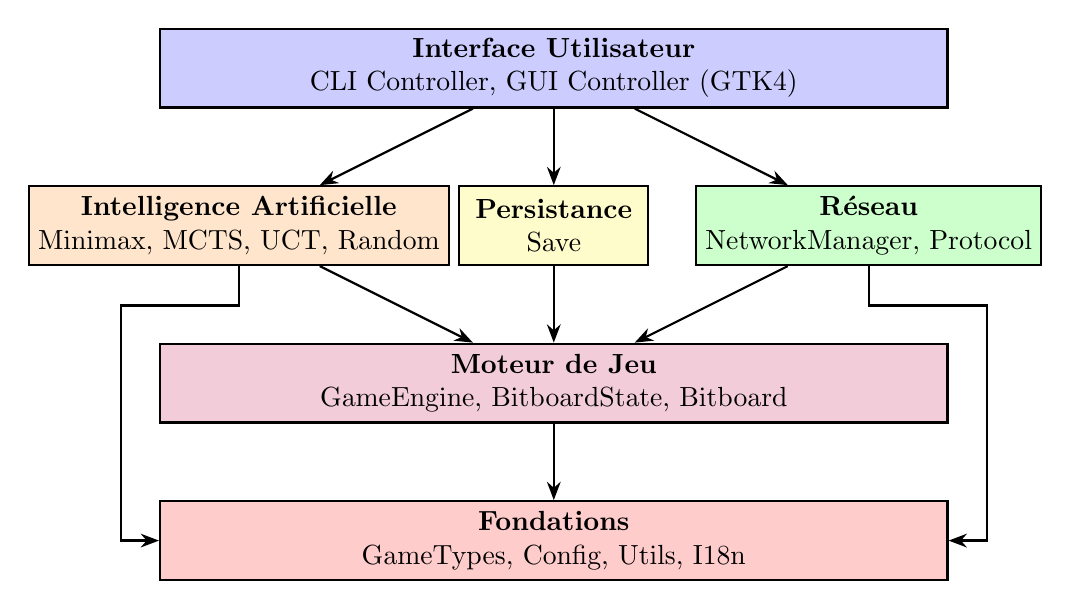
\begin{tikzpicture}[
    layer/.style={rectangle, draw, thick, minimum height=1cm, align=center},
    arrow/.style={->, >=Stealth, thick}
]
% Layers
\node[layer, fill=blue!20, minimum width=10cm] (ui) at (0,2) {\textbf{Interface Utilisateur} \\ CLI Controller, GUI Controller (GTK4)};

\node[layer, fill=orange!20, minimum width=3.2cm] (ai) at (-4,0) {\textbf{Intelligence Artificielle} \\ Minimax, MCTS, UCT, Random};
\node[layer, fill=yellow!20, minimum width=2.4cm] (save) at (0,0) {\textbf{Persistance} \\ Save};
\node[layer, fill=green!20, minimum width=3.2cm] (net) at (4,0) {\textbf{Réseau} \\ NetworkManager, Protocol};

\node[layer, fill=purple!20, minimum width=10cm] (engine) at (0,-2) {\textbf{Moteur de Jeu} \\ GameEngine, BitboardState, Bitboard};

\node[layer, fill=red!20, minimum width=10cm] (core) at (0,-4) {\textbf{Fondations} \\ GameTypes, Config, Utils, I18n};

% Arrows from UI to middle layer
\draw[arrow] (ui) -- (ai);
\draw[arrow] (ui) -- (save);
\draw[arrow] (ui) -- (net);

% Arrows from middle layer to Engine
\draw[arrow] (ai) -- (engine);
\draw[arrow] (save) -- (engine);
\draw[arrow] (net) -- (engine);

% Arrow from Engine to Core
\draw[arrow] (engine) -- (core);

% Arrows from middle layer to Core (contournement extérieur)
\draw[arrow] (ai.south) -- ++(0,-0.5) -- ++(-1.5,0) |- (core.west);
\draw[arrow] (net.south) -- ++(0,-0.5) -- ++(1.5,0) |- (core.east);

\end{tikzpicture}
\caption{Architecture en couches du projet. Les flèches représentent les dépendances~: chaque module dépend uniquement des couches inférieures, garantissant testabilité et maintenabilité.}
\label{fig:arch-layers}
\end{figure}

Le moteur de jeu constitue le \textbf{noyau pur} de l'application~: totalement indépendant de l'affichage et du réseau, il expose une API pour la manipulation de l'état du jeu. Les modules d'IA interrogent ce moteur via l'interface \texttt{BitboardState} pour des calculs haute performance, tandis que les contrôleurs manipulent le \texttt{GameState}. Le réseau et l'IA communiquent avec l'interface via un système de \textbf{callbacks}, évitant ainsi toute dépendance cyclique.
\subsection{Architecture du module IA}
\label{sec:ia-arch-detail}

\subsubsection{Le patron Factory et la table virtuelle}

Le système d'IA repose sur deux abstractions complémentaires~: une \textbf{usine de création} (\texttt{ai\_factory.c}) et une \textbf{interface polymorphe} (\texttt{AI\_Interface}). Cette architecture permet d'instancier dynamiquement différents types d'IA à partir de chaînes de caractères, sans couplage statique entre le contrôleur et les implémentations concrètes.

\begin{figure}[H]
\centering
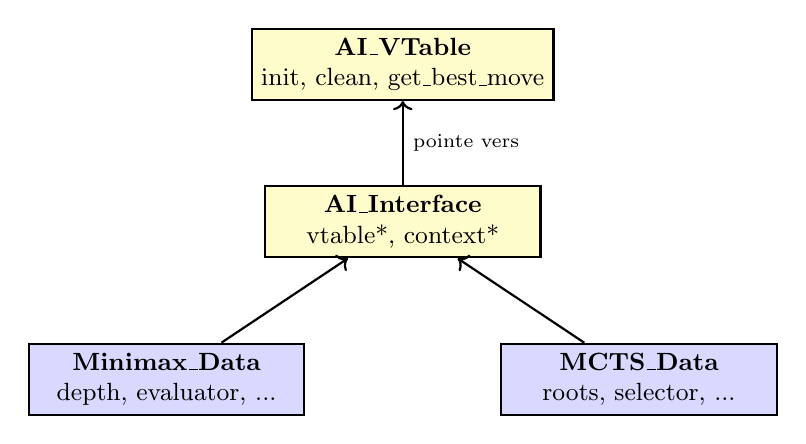
\begin{tikzpicture}[
    class/.style={rectangle, draw, thick, minimum width=3.5cm, minimum height=0.8cm, align=center, font=\small},
    interface/.style={class, fill=yellow!20},
    concrete/.style={class, fill=blue!15}
]

\node[interface] (vtable) at (0,0) {\textbf{AI\_VTable} \\ init, clean, get\_best\_move};
\node[interface] (iface) at (0,-2) {\textbf{AI\_Interface} \\ vtable*, context*};
\node[concrete] (minimax) at (-3,-4) {\textbf{Minimax\_Data} \\ depth, evaluator, ...};
\node[concrete] (mcts) at (3,-4) {\textbf{MCTS\_Data} \\ roots, selector, ...};

\draw[->, thick] (iface) -- node[right, font=\scriptsize] {pointe vers} (vtable);
\draw[->, thick] (minimax) -- (iface);
\draw[->, thick] (mcts) -- (iface);

\end{tikzpicture}
\caption{Diagramme UML simplifié du système d'IA. Chaque IA concrète implémente les trois méthodes de la VTable et stocke son état privé dans \texttt{context}.}
\end{figure}

L'usine maintient un registre statique des IA disponibles~:

\begin{lstlisting}[language=C, caption=Extrait du registre de l'usine]
static const AI_RegistryEntry AI_REGISTRY[] = {
    { "random", create_random_ai },
    { "minimax", create_minimax_ai },
    { "iterative", create_minimax_ai }, // alias
    { "mcts", create_mcts_ai }
};
\end{lstlisting}

Lors de l'appel à \texttt{create\_ai("mcts", params)}, l'usine~:
\begin{enumerate}
    \item Recherche "mcts" dans le registre
    \item Invoque \texttt{create\_mcts\_ai(\&ai)} pour initialiser la VTable
    \item Appelle \texttt{ai.vtable->init(\&ai, \&params)} pour construire le contexte
    \item Retourne l'interface complète
\end{enumerate}

Cette indirection permet d'ajouter de nouvelles IA sans modifier le code appelant. Par exemple, ajouter une IA basée sur un solveur de preuve nécessite uniquement~:
\begin{itemize}
    \item Créer \texttt{src/ai/solver/solver.c} avec les fonctions \texttt{solver\_init}, \texttt{solver\_clean}, \texttt{solver\_get\_best\_move}
    \item Ajouter \texttt{\{ "solver", create\_solver\_ai \}} au registre
\end{itemize}

\subsubsection{Injection de dépendances par ConfigMap}

Les paramètres de configuration sont transmis sous forme de dictionnaire clé-valeur dynamique~:

\begin{lstlisting}[language=C, caption=Exemple d'utilisation du ConfigMap]
Param params[] = {
    { "depth", "5" },
    { "evaluator", "qd&kd" },
    { "forward_pruning", "1" }
};
ConfigMap cfg = { 3, params };
AI_Interface ai = create_ai("minimax", cfg);
\end{lstlisting}

La macro générique \texttt{check\_param} utilise \texttt{\_Generic} (C11) pour dispatcher automatiquement vers la fonction de parsing appropriée selon le type de la cible~:

\begin{lstlisting}[language=C]
int depth = 3;
bool pruning = false;
const char* eval = "me";

check_param(params[0], "depth", &depth);         // -> int
check_param(params[1], "evaluator", &eval);     // -> const char**
check_param(params[2], "forward_pruning", &pruning); // -> bool
\end{lstlisting}

Cette approche élimine le besoin de structures de configuration rigides et permet l'ajout de nouveaux paramètres sans casser la compatibilité binaire.

\subsubsection{Découplage évaluateurs et sélecteurs}

Les heuristiques d'évaluation (Minimax) et les stratégies de sélection (MCTS) sont également découplées par des interfaces~:

\begin{lstlisting}[language=C, caption=Interface des évaluateurs]
typedef float (*Evaluator)(const BitboardState* state);

Evaluator get_evaluator(EvaluatorType type) {
    switch (type) {
        case EVAL_ME: return eval_me;
        case EVAL_RTH: return eval_rth;
        case EVAL_QD_KD: return eval_qdkd;
        default: return eval_me;
    }
}
\end{lstlisting}

Les sélecteurs MCTS suivent un patron similaire avec une VTable dédiée (\texttt{ISelector\_VTable}) permettant de basculer entre UCT et PUCT sans recompiler le cœur de MCTS.

\subsection{Le moteur de jeu}

Le moteur de jeu a été architecturé comme le modèle pur de l'application.
Il est totalement indépendant du système d'entrée/sortie~: son code interne
ne contient aucune instruction d'affichage sur la sortie standard, n'écrit
pas dans des fichiers, et ne tente aucune lecture asynchrone sur le clavier.
Il communique avec l'extérieur exclusivement via une API publique définie
dans son en-tête.

Grâce à cette architecture de composants isolés, le même moteur de jeu
peut arbitrer une partie locale dans le terminal, valider des coups
asynchrones sur le serveur réseau, ou simuler des parties virtuelles pour
l'IA, sans nécessiter la moindre modification de sa structure interne.

%------------------------------------------------------------------------------
% SECTION 3.4 - Architecture du module réseau
%------------------------------------------------------------------------------
 
\subsection{Architecture du module réseau}
\label{sec:network-arch}
 
L'architecture du module réseau repose sur trois piliers conceptuels~: une
façade centralisée masquant la complexité des sockets, un modèle événementiel
mono-threadé basé sur le multiplexage, et un système de rappels découplant
le cœur réseau des interfaces utilisateur. La figure~\ref{fig:network-composition}
illustre l'organisation générale de ces composants.
 
% DIAGRAMME 1 : Composition du NetworkManager
\begin{figure}[H]
\centering
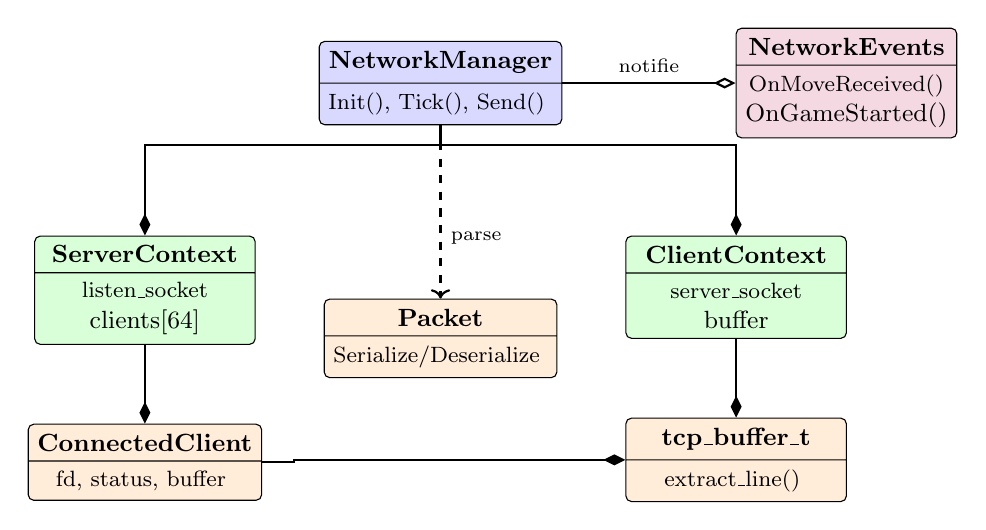
\begin{tikzpicture}[
    node distance=1.2cm and 1.8cm,
    class/.style={
        rectangle split,
        rectangle split parts=2,
        draw,
        rounded corners=2pt,
        minimum width=2.8cm,
        font=\small,
        align=center
    },
    facade/.style={class, fill=blue!15},
    context/.style={class, fill=green!15},
    data/.style={class, fill=orange!15},
    interface/.style={class, fill=purple!15},
    composition/.style={-{Diamond[fill=black]}, thick},
    aggregation/.style={-{Diamond[fill=white]}, thick},
    dependency/.style={->, dashed, thick},
]
 
% NetworkManager (Façade)
\node[facade] (nm) {
    \textbf{NetworkManager}
    \nodepart{second}
    \footnotesize
    Init(), Tick(), Send()
};
 
% Contextes
\node[context, below left=1.4cm and 0.8cm of nm] (server) {
    \textbf{ServerContext}
    \nodepart{second}
    \footnotesize
    listen\_socket\\clients[64]
};
 
\node[context, below right=1.4cm and 0.8cm of nm] (client) {
    \textbf{ClientContext}
    \nodepart{second}
    \footnotesize
    server\_socket\\buffer
};
 
% ConnectedClient
\node[data, below=1cm of server] (cc) {
    \textbf{ConnectedClient}
    \nodepart{second}
    \footnotesize
    fd, status, buffer
};
 
% tcp_buffer_t
\node[data, below=1cm of client] (buffer) {
    \textbf{tcp\_buffer\_t}
    \nodepart{second}
    \footnotesize
    extract\_line()
};
 
% NetworkEvents (Observateur)
\node[interface, right=2.2cm of nm] (events) {
    \textbf{NetworkEvents}
    \nodepart{second}
    \footnotesize
    OnMoveReceived()\\OnGameStarted()
};
 
% Packet
\node[data, below=2.2cm of nm] (packet) {
    \textbf{Packet}
    \nodepart{second}
    \footnotesize
    Serialize/Deserialize
};
 
% Relations
\draw[composition] (nm.south) -- ++(0,-0.25) -| (server.north);
\draw[composition] (nm.south) -- ++(0,-0.25) -| (client.north);
\draw[composition] (server.south) -- (cc.north);
\draw[composition] (client.south) -- (buffer.north);
\draw[composition] (cc.east) -- ++(0.4,0) |- (buffer.west);
\draw[aggregation] (nm.east) -- node[above, font=\scriptsize] {notifie} (events.west);
\draw[dependency] (nm.south) -- node[right, font=\scriptsize, pos=0.65] {parse} (packet.north);
 
\end{tikzpicture}
\caption{Diagramme de composition du \texttt{NetworkManager}. La façade possède
au plus un contexte serveur \textbf{ou} client (exclusion mutuelle). Chaque
client embarque son propre tampon TCP. Légende~: $\blacklozenge$ composition,
$\lozenge$ agrégation, trait pointillé = dépendance.}
\label{fig:network-composition}
\end{figure}
 
\subsubsection{La façade \texttt{NetworkManager}}
\label{subsec:facade}
 
\paragraph{Principe architectural.}
Le module réseau expose une unique structure publique --- \texttt{NetworkManager}
--- qui encapsule l'intégralité de la logique de communication. Les couches
supérieures (CLI, GUI) n'ont jamais besoin de manipuler directement les
descripteurs de fichiers, les structures d'adresses réseau, ni les tampons
de framing. Ce masquage strict de l'information garantit que toute évolution
interne (passage à TLS, changement de protocole) n'impacte pas le code client.

L'initialisation de la façade illustre cette encapsulation~:

\begin{lstlisting}[language=C, caption=Initialisation du NetworkManager]
void NetworkManager_Init(NetworkManager *manager, NetworkEvents callbacks) {
  manager->current_mode = NET_MODE_NONE;
  manager->server_ctx = NULL;
  manager->client_ctx = NULL;
  manager->callbacks = callbacks;  // Injection des rappels
}
\end{lstlisting}
 
\paragraph{Dualité serveur/client.}
Le \texttt{NetworkManager} peut fonctionner en trois modes mutuellement
exclusifs~: inactif, serveur ou client. En mode serveur, il alloue un
\texttt{ServerContext} contenant la socket d'écoute, le tableau des 64 slots
clients avec leurs tampons TCP respectifs, le tableau des 32 parties actives,
et le contexte de découverte UDP. En mode client, il alloue un
\texttt{ClientContext} minimaliste contenant uniquement la socket de connexion
au serveur et son tampon de réception. Cette ségrégation mémoire évite toute
confusion entre les rôles et permet une libération ciblée des ressources.
 
\subsubsection{Le multiplexage asynchrone avec \texttt{poll()}}
\label{subsec:multiplexing}
 
\paragraph{Choix du modèle événementiel.}
Pour gérer simultanément jusqu'à 64 connexions sans threads, nous avons opté
pour le multiplexage d'entrées/sorties via l'appel système \texttt{poll()}.
Trois alternatives existaient~: \texttt{select()}, limité à 1\,024 descripteurs
et utilisant des masques de bits peu pratiques~; \texttt{epoll()}, plus
performant mais spécifique à Linux~; et \texttt{poll()}, offrant une interface
portable POSIX avec des performances adaptées à notre charge. Le modèle
mono-threadé élimine par construction les conditions de course et la nécessité
de verrous, simplifiant considérablement le raisonnement sur la correction
du code.
 
\paragraph{Boucle non bloquante.}
La fonction \texttt{NetworkManager\_Tick()}, appelée à chaque itération de la
boucle principale, invoque \texttt{poll()} avec un timeout nul. Ce paramétrage
rend l'appel instantanément retourné~: si des données sont disponibles, elles
sont traitées~; sinon, le contrôle revient immédiatement à l'appelant. Cette
conception permet à l'interface de continuer à traiter d'autres événements
(saisie clavier, rafraîchissement graphique) entre deux cycles réseau.

\begin{lstlisting}[language=C, caption=Tick serveur avec poll() non bloquant]
static void handle_server_tick(NetworkManager *manager, ServerContext *ctx) {
  int poll_count = poll(ctx->fds, MAX_CLIENTS + 1, POLL_TIMEOUT_IMMEDIATE);
  
  if (poll_count > 0) {
    if (ctx->fds[LISTEN_SOCKET_INDEX].revents & POLLIN)
      handle_server_new_connection(ctx);
    
    for (int i = FIRST_CLIENT_INDEX; i <= MAX_CLIENTS; i++) {
      if (ctx->fds[i].fd != INVALID_SOCKET &&
          (ctx->fds[i].revents & (POLLIN | POLLHUP | POLLERR)))
        handle_server_client_data(manager, ctx, i);
    }
  }
}
\end{lstlisting}
 
\paragraph{Double multiplexage dans la boucle CLI.}
La boucle principale du CLI illustre une application avancée de ce modèle~:
elle doit surveiller simultanément deux sources d'événements indépendantes
--- le réseau et le clavier. Plutôt que de créer deux threads ou de bloquer
sur l'une des sources, nous utilisons deux appels \texttt{poll()} distincts
à chaque itération~: le premier interroge les sockets réseau avec un timeout
nul (traitement immédiat des paquets entrants), le second interroge
\texttt{stdin} avec un court timeout permettant la saisie de commandes. Cette
architecture permet au joueur de taper des commandes tout en recevant
instantanément les coups de l'adversaire, simulant un parallélisme sans les
risques inhérents à la programmation concurrente. La figure~\ref{fig:seq_multiplexing}
en annexe illustre cette alternance temporelle.
 
\subsubsection{Le patron Observateur pour le découplage}
\label{subsec:observer}
 
\paragraph{Interface de rappels.}
La communication entre le module réseau et les couches supérieures est régie
par le patron \textit{Observer}. À l'initialisation, le \texttt{NetworkManager}
reçoit une structure \texttt{NetworkEvents} contenant neuf pointeurs de
fonctions couvrant tous les événements significatifs~: réception d'un coup,
connexion ou déconnexion d'un joueur, réception d'une invitation, démarrage
d'une partie, erreur protocolaire, expiration du temps de réflexion, et
réception d'une liste de joueurs.
 
\paragraph{Inversion de contrôle.}
Lorsque le réseau reçoit un coup valide, il se contente d'invoquer le rappel
\texttt{OnMoveReceived(move)} sans connaître l'identité de l'appelant. C'est
la couche d'interface qui décide de la réaction appropriée~: le CLI met à jour
l'affichage textuel du plateau et réaffiche le prompt, tandis que la GUI
redessine les cases concernées via les primitives GTK. Cette inversion de
contrôle garantit que le module réseau reste totalement indépendant des
interfaces utilisateur~: les fichiers d'implémentation CLI et GUI fournissent
chacun leur propre jeu de rappels sans qu'une seule ligne du cœur réseau
n'ait été modifiée.
 
\subsubsection{Routage des paquets et arbitrage serveur}
\label{subsec:routing}
 
\paragraph{Architecture du routeur.}
Une fois un paquet désérialisé, il est acheminé vers un gestionnaire dédié
via une structure de sélection indexée par le type de paquet. Cette conception
respecte le principe ouvert/fermé~: ajouter un nouveau type de message
nécessite uniquement l'ajout d'un cas dans le gestionnaire, sans modifier
la logique de routage existante.

\begin{lstlisting}[language=C, caption=Routage des paquets par type]
void handle_server_packet(NetworkManager *manager, ServerContext *ctx,
                          int client_index, Packet *pkt) {
  switch (pkt->type) {
    case C2S_JOIN:   process_join_packet(manager, ctx, client_index, pkt->payload); break;
    case C2S_INVITE: process_invite_packet(manager, ctx, client_index, pkt->payload); break;
    case C2S_MOVE:   process_move_packet(manager, ctx, client_index, pkt->payload); break;
    case C2S_HEARTBEAT: break;  // Mise a jour silencieuse du timestamp
    // ... autres cas
    default: printf("[SERVER] Unmanaged packet (Type: %d)\n", pkt->type);
  }
}
\end{lstlisting}
 
\paragraph{Arbitrage anti-triche.}
Le serveur ne se contente pas de relayer aveuglément les coups entre joueurs.
Avant tout transfert, il maintient une copie locale du plateau pour chaque
partie active et valide la légalité de chaque coup reçu. Si un coup est
déterminé illégal par le moteur de jeu, il est rejeté avec un message d'erreur
explicite envoyé au client fautif, et l'adversaire n'est jamais notifié de
cette tentative. Ce mécanisme garantit qu'un client malveillant ou bogué ne
peut pas corrompre l'état de jeu de son adversaire ni obtenir un avantage
indu.

\begin{lstlisting}[language=C, caption=Validation anti-triche des coups]
// Extrait de process_move_packet()
GameState *server_board = &ctx->active_games[game_idx];

if (is_move_legal(server_board, parsed_move)) {
  apply_move(server_board, parsed_move);  // MAJ plateau arbitre
  // Relais vers l'adversaire...
} else {
  printf("[ANTI-CHEAT] Client %d tried illegal move\n", client_index);
  send_error(manager, client_index, "Illegal move detected!");
}
\end{lstlisting}
 
\paragraph{Routage par identifiant de partie.}
Chaque partie active possède un identifiant unique attribué séquentiellement
par le serveur. Lorsqu'un client envoie un coup, le serveur consulte son
champ \texttt{game\_id} pour identifier la partie concernée, puis parcourt
les clients connectés pour trouver celui partageant le même identifiant avec
un statut «~en jeu~». Cette recherche, bien que linéaire dans le pire cas
($\mathcal{O}(n)$ où $n$ est le nombre de clients), reste négligeable en
pratique car le nombre de clients actifs est borné.

\subsubsection{Sérialisation et framing TCP}
\label{subsec:serialization}

\paragraph{Format des paquets.}
Chaque paquet suit le format textuel \texttt{"TYPE|PAYLOAD\textbackslash{}n"}. La sérialisation et désérialisation s'effectuent en temps linéaire par rapport à la taille du message~:

\begin{lstlisting}[language=C, caption=Sérialisation des paquets]
int SerializePacket(const Packet *pkt, char *buffer_out, size_t max_len) {
  return snprintf(buffer_out, max_len, "%d|%s\n", pkt->type, pkt->payload);
}
\end{lstlisting}

\paragraph{Extraction des messages.}
Le tampon TCP accumule les fragments jusqu'à réception d'un délimiteur \texttt{'\textbackslash{}n'}. L'extraction utilise \texttt{memchr()} pour la recherche et \texttt{memmove()} pour la compaction~:

\begin{lstlisting}[language=C, caption=Extraction d'une ligne du tampon TCP]
int tcp_buffer_extract_line(tcp_buffer_t *buf, char *out_msg, size_t max_len) {
  char *newline = memchr(buf->data, '\n', buf->length);
  if (newline == NULL) return EXTRACT_NO_MSG;
  
  size_t msg_len = newline - buf->data;
  memcpy(out_msg, buf->data, msg_len);
  out_msg[msg_len] = '\0';
  
  size_t remaining = buf->length - msg_len - 1;
  memmove(buf->data, newline + 1, remaining);  // Compaction
  buf->length = remaining;
  return EXTRACT_SUCCESS;
}
\end{lstlisting}

\subsection{Le module d'interface graphique (GUI)}
\label{sec:gui-arch}

L'architecture de l'interface graphique a été pensée pour séparer la logique métier de la présentation visuelle, s'inspirant du patron Modèle-Vue-Contrôleur (MVC).

% DIAGRAMME ARCHITECTURE GUI
\begin{figure}[H]
\centering
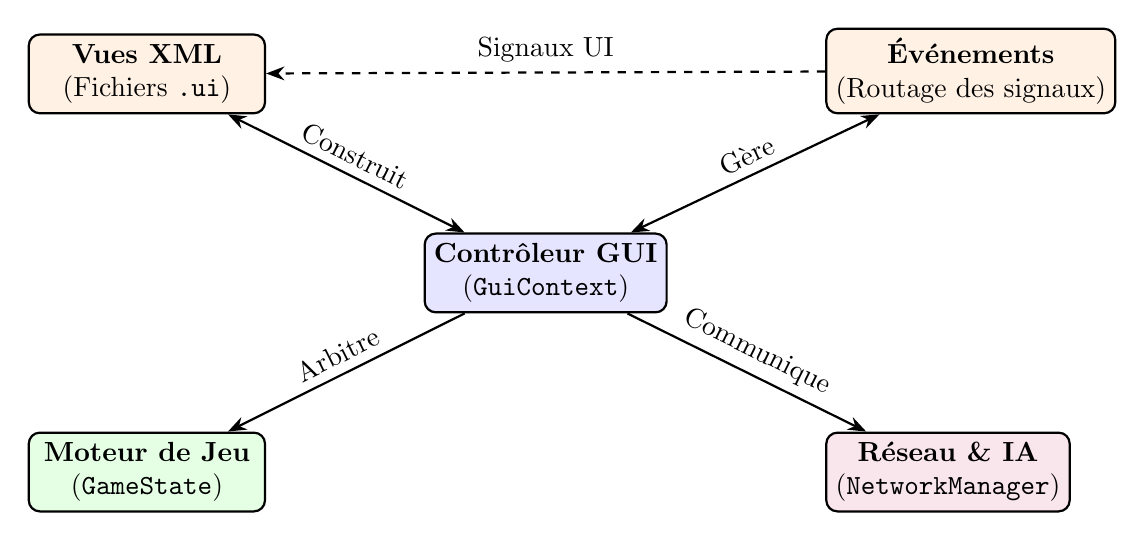
\begin{tikzpicture}[
    node distance=1.5cm and 2cm,
    module/.style={rectangle, draw, rounded corners, fill=blue!10, thick, minimum width=3cm, minimum height=1cm, align=center},
    view/.style={rectangle, draw, rounded corners, fill=orange!10, thick, minimum width=3cm, minimum height=1cm, align=center},
    arrow/.style={->, thick, >=Stealth}
]

% Nodes
\node[module] (controller) {\textbf{Contrôleur GUI}\\(\texttt{GuiContext})};
\node[view, above left=of controller] (pages) {\textbf{Vues XML}\\(Fichiers \texttt{.ui})};
\node[view, above right=of controller] (callbacks) {\textbf{Événements}\\(Routage des signaux)};
\node[module, fill=green!10, below left=of controller] (engine) {\textbf{Moteur de Jeu}\\(\texttt{GameState})};
\node[module, fill=purple!10, below right=of controller] (network) {\textbf{Réseau \& IA}\\(\texttt{NetworkManager})};

% Arrows
\draw[arrow, <->] (controller) -- node[above, sloped] {Construit} (pages);
\draw[arrow, <->] (controller) -- node[above, sloped] {Gère} (callbacks);
\draw[arrow, dashed] (callbacks) -- node[above] {Signaux UI} (pages);
\draw[arrow] (controller) -- node[above, sloped] {Arbitre} (engine);
\draw[arrow] (controller) -- node[above, sloped] {Communique} (network);

\end{tikzpicture}
\caption{Architecture du module graphique~: le contrôleur orchestre les vues asynchrones, le réseau et le modèle de jeu.}
\label{fig:gui_architecture}
\end{figure}

\subsubsection{Séparation vue/logique via XML}

L'interface visuelle est définie dans des fichiers de description déclarative (XML). Cette séparation stricte entre définition de l'interface et logique procédurale présente deux avantages~: la modification de la mise en page d'un écran est indépendante de la logique applicative, et l'initialisation du code se concentre purement sur la connexion des actions (\textit{event binding}). Les ressources graphiques sont compilées dans un binaire embarqué au démarrage (\textit{Resource Bundle}), rendant l'exécutable autonome.

\subsubsection{Le contrôleur asynchrone et la Main Loop}

Le point central de l'architecture GUI est son contrôleur. Le système de fenêtrage reposant sur une boucle d'événements bloquante (\textit{Main Loop}), toute boucle d'attente classique (pour écouter le réseau ou calculer un coup d'IA) gèlerait l'interface. Le contrôleur résout ce problème en intégrant l'écoute réseau et l'IA sous forme de tâches asynchrones planifiées par le séquenceur de l'interface (\textit{timeouts}). Réseau, IA et rendu graphique coopèrent ainsi de manière fluide sur le même fil d'exécution.

\subsubsection{Navigation avec GtkStack}

La structure de navigation repose sur un conteneur dynamique gérant un empilement de vues (menu principal, configuration, jeu, lobby réseau). Le couplage lâche, permis par le stockage de balises de destination directement dans les propriétés des boutons, permet de définir la navigation globale depuis les vues XML, sans multiplier les fonctions de routage spécifiques dans le contrôleur.

\subsubsection{Le plateau de jeu et la validation retardée}

Le déplacement d'une pièce suit un protocole strict en trois étapes~: sélection de la pièce, déplacement temporaire en mémoire locale pour assurer le retour visuel, puis confirmation finale par le tir de la flèche. La méthode de mutation officielle de l'état (\texttt{apply\_move}) n'est sollicitée qu'à l'issue de cette transaction. Cette approche transactionnelle garantit que le moteur de jeu central (et son historique d'annulation) n'enregistre jamais d'états partiels ou de coups incomplets.


\subsection{Module CLI}

Le fichier de commandes CLI constitue la base de l'interface en ligne de
commande. Sa fonction principale reçoit le texte saisi par le joueur et
utilise une série de comparaisons pour identifier l'action demandée. Des
constantes symboliques remplacent systématiquement les longueurs de chaînes
codées en dur, ce qui facilite la maintenance lors de modifications des noms
de commandes.

Pour éviter les variables globales, l'ensemble du contexte est centralisé
dans une structure \texttt{CliContext} transmise à chaque fonction. Cette
structure regroupe le pointeur vers la partie en cours, les réglages, l'état
de navigation (menu principal, partie réseau, statut absent), le gestionnaire
de réseau, ainsi que des métadonnées de gestion du temps et de l'IA.
Ce contexte permet par exemple de bloquer la commande de déplacement si
le joueur se trouve en lobby réseau, ou d'empêcher le lancement d'un second
serveur si un premier est déjà actif.

\subsection{Architecture des contrôleurs}
\label{sec:controller-arch}
 
Les contrôleurs CLI et GUI partagent une responsabilité commune~: orchestrer les interactions entre l'utilisateur, le moteur de jeu, l'IA et le réseau. Cependant, leurs modèles d'exécution diffèrent fondamentalement.
 
\subsubsection{Le contrôleur CLI~: boucle événementielle hybride}
 
Le contrôleur CLI implémente une boucle principale non bloquante qui doit surveiller simultanément deux sources d'événements indépendantes~: le réseau et le clavier. Plutôt que de créer deux threads, nous utilisons un double multiplexage avec \texttt{poll()}~:
 
\begin{lstlisting}[language=C, caption=Boucle principale du contrôleur CLI]
void run_interactive_mode(game_config_t *config) {
  CliContext *ctx = calloc(1, sizeof(CliContext));
  NetworkManager_Init(&ctx->net_manager, create_cli_network_events(ctx));
  
  // Configuration de readline en mode callback
  rl_callback_handler_install("", linehandler);
  
  struct pollfd fds[1];
  fds[0].fd = STDIN_FILENO;
  fds[0].events = POLLIN;
  
  while (ctx->game_running) {
    // 1. Tick reseau (poll interne avec timeout=0)
    NetworkManager_Tick(ctx->net_manager);
    
    // 2. Verification fin de partie
    if (is_game_over(ctx->current_game, ctx->current_game->current_player)) {
      handle_game_over(ctx);
      continue;
    }
    
    // 3. Tour de l'IA si applicable
    if (is_it_ai_turn(ctx->config, ctx->current_game->current_player)) {
      execute_ai_turn(ctx);
    }
    
    // 4. Gestion du timeout reseau synchronise
    handle_network_timeout(ctx);
    
    // 5. Poll clavier avec timeout court (100ms)
    int poll_res = poll(fds, 1, POLL_STDIN_TIMEOUT_MS);
    if (poll_res > 0 && (fds[0].revents & POLLIN)) {
      rl_callback_read_char();
    }
  }
  
  cleanup_resources(ctx);
}
\end{lstlisting}
 
Cette architecture permet au joueur de taper des commandes tout en recevant instantanément les coups de l'adversaire, simulant un parallélisme sans les risques de la programmation concurrente.
 
\subsubsection{Dispatch des commandes CLI}
 
Les commandes saisies sont routées via une fonction de dispatch centralisée. Le contrôleur vérifie d'abord le contexte actuel (menu principal, lobby réseau, partie en cours) avant d'exécuter l'action~:
 
\begin{lstlisting}[language=C, caption=Extrait du dispatch des commandes CLI]
void handle_command(const char *input, CliContext *ctx) {
  // Commandes toujours disponibles
  if (strncmp(input, "help", 4) == 0) {
    execute_help(ctx);
    return;
  }
  if (strncmp(input, "quit", 4) == 0) {
    execute_quit(ctx);
    return;
  }
  
  // Commandes dependantes du contexte
  if (ctx->in_main_menu) {
    // Seules new, load, server start, join sont autorisees
    if (strncmp(input, "new", 3) == 0) {
      execute_new_game(ctx);
    } else if (strncmp(input, "server start", 12) == 0) {
      execute_server_start(ctx, input + 12);
    }
    // ...
  } else if (ctx->in_network_match) {
    // En partie reseau : uniquement les coups et commandes de jeu
    if (is_move_notation(input)) {
      execute_network_move(ctx, input);
    }
  } else {
    // Partie locale : toutes les commandes de jeu
    handle_local_game_command(ctx, input);
  }
}
\end{lstlisting}
 
\subsubsection{Le contrôleur GUI~: intégration asynchrone avec GLib}
 
Le contrôleur graphique s'intègre à la boucle d'événements GTK (\textit{Main Loop}) via des callbacks et des timeouts planifiés. L'IA ne peut pas calculer de manière bloquante car cela gèlerait l'interface~:
 
\begin{lstlisting}[language=C, caption=Intégration asynchrone de l'IA dans le contrôleur GUI]
void guiHandlePlayerMove(AppContext *ctx, Move move) {
  if (!is_move_legal(ctx->gameState, move)) {
    g_print("Error: Engine rejected the move.\n");
    return;
  }
  
  apply_move(ctx->gameState, move);
  clearHighlights(ctx);
  drawBoard(ctx);
  ctx->currentPhase = PHASE_MOVE_QUEEN;
  
  if (is_game_over(ctx->gameState, ctx->gameState->current_player)) {
    show_game_over_dialog(ctx);
    return;
  }
  
  // Planification asynchrone du tour IA
  if (is_it_ai_turn(ctx->gameConfig, ctx->gameState->current_player)) {
    // Delai de 50ms pour laisser le rendu se terminer
    g_timeout_add(50, guiAIPlayTurn, ctx);
  }
}
 
static gboolean guiAIPlayTurn(gpointer user_data) {
  AppContext *ctx = (AppContext *)user_data;
  
  AI_Interface *ai = get_current_ai(ctx);
  Move ai_move = ai->vtable->get_best_move(ai, *(ctx->gameState));
  
  guiHandlePlayerMove(ctx, ai_move);
  
  return G_SOURCE_REMOVE;  // Execution unique
}
\end{lstlisting}
 
Le callback \texttt{guiAIPlayTurn} est exécuté par le séquenceur GLib après le délai spécifié, permettant au rendu graphique de se terminer avant le calcul de l'IA.
%==============================================================================
\section{Explication approfondie}
\label{sec:deep}
%==============================================================================

 
%------------------------------------------------------------------------------
% SECTION 4.1 - Cycle de vie des connexions
%------------------------------------------------------------------------------
 
%------------------------------------------------------------------------------
% SECTION 4.1 - REMPLACE l'ancienne section "Cycle de vie des connexions"
%------------------------------------------------------------------------------
 
\subsection{Fonctionnalité réseau~: Système d'invitations et machine à états (F40)}
\label{subsec:network-invitations}
 
\subsubsection{Prérequis et problème}
 
Le cahier des charges (F40) impose un système complet d'invitations permettant aux joueurs de se défier dans le lobby. Ce système doit gérer plusieurs cas complexes~: un joueur peut être indisponible (\texttt{AWAY}), déjà en partie (\texttt{INGAME}), ou en attente de réponse (\texttt{WAITGAME}). Les invitations doivent expirer automatiquement après 5 minutes, et toute transition d'état invalide doit être rejetée avec un message explicite.
 
\subsubsection{Solution implémentée~: machine à états finis}
 
Nous avons modélisé le cycle de vie d'un client par un automate fini à cinq états. Chaque transition est gardée par des vérifications explicites~:
 
\begin{lstlisting}[language=C, caption=Énumération des statuts clients]
typedef enum {
  CLIENT_STATUS_CONNECTED,  // TCP etabli, attente JOIN
  CLIENT_STATUS_IDLE,       // Dans le lobby, disponible
  CLIENT_STATUS_AWAY,       // Indisponible temporairement
  CLIENT_STATUS_WAITGAME,   // Invitation en attente
  CLIENT_STATUS_INGAME      // Partie en cours
} ClientStatus;
\end{lstlisting}
 
\paragraph{Traitement d'une invitation.}
Lorsqu'un joueur envoie une invitation, le serveur vérifie l'éligibilité via des gardes d'état~:
 
\begin{lstlisting}[language=C, caption=Gardes de transition pour les invitations]
// Extrait de process_invite_packet()
if (ctx->clients[sender_index].status != CLIENT_STATUS_IDLE) {
  send_error(manager, sender_index, "You must be IDLE to invite.");
  return;
}
if (ctx->clients[target_id].status == CLIENT_STATUS_AWAY) {
  send_error(manager, sender_index, "Player is currently AWAY.");
  return;
}
// Transitions d'etat apres validation
ctx->clients[sender_index].status = CLIENT_STATUS_WAITGAME;
ctx->clients[target_id].pending_invite_from = sender_index;
\end{lstlisting}
 
\paragraph{Expiration automatique.}
À chaque tick serveur, les invitations pendantes sont vérifiées. Une invitation non répondue après 300 secondes déclenche le retour au statut \texttt{IDLE} pour les deux joueurs avec notification explicite.
 
\subsubsection{Garanties de cohérence}
 
Cette implémentation garantit trois propriétés~: \textbf{déterminisme} (chaque paquet produit exactement une transition ou un rejet), \textbf{isolation} (un joueur en partie ne peut recevoir d'invitations), et \textbf{récupération automatique} (les timeouts libèrent les ressources bloquées).
 

\subsection{Fonctionnalité 4~: Approfondissement itératif avec contrainte de temps}
\label{subsec:iterative-deepening}

\subsubsection{Prérequis et problème}

L'algorithme Minimax classique explore l'arbre de jeu jusqu'à une profondeur fixe $d$, puis retourne le meilleur coup trouvé. Cette approche présente un défaut majeur~: si $d$ est trop grand, le calcul peut dépasser le temps imparti, ne retournant aucun coup valide. Si $d$ est trop petit, l'IA joue de manière myope. Le cahier des charges (F34) impose donc un mécanisme garantissant le retour du \textbf{meilleur coup trouvé à la profondeur maximale complétée} avant l'expiration du délai.

\subsubsection{Solution implémentée~: Iterative Deepening}

L'approfondissement itératif consiste à explorer l'arbre en profondeur croissante ($d = 1, 2, 3, \ldots$) jusqu'à épuisement du temps. À chaque itération complète, le meilleur coup est mis à jour. Si le temps expire en milieu d'exploration, le coup de l'itération précédente est retourné.

\paragraph{Implémentation.}
La fonction \texttt{minimax\_get\_best\_move} contient une boucle principale~:

\begin{lstlisting}[language=C, caption=Boucle d'approfondissement itératif]
Move best_move_overall = available_moves[0];

for (int d = 1; d <= data->max_depth; d++) {
    if (get_time_ms() - start_time >= data->time_limit)
        break;
    
    // Tri des coups pour placer le meilleur de l'iteration
    // precedente en tete (ameliore le pruning)
    if (d > 1)
        sort_moves(count, best_move_overall, available_moves);
    
    Move move_at_depth = run_root_search(data, &root_state, d, 
                                         start_time, available_moves, count);
    
    // Sauvegarde uniquement si l'iteration s'est terminee
    if (get_time_ms() - start_time < data->time_limit) {
        best_move_overall = move_at_depth;
    }
}

return best_move_overall;
\end{lstlisting}

\paragraph{Optimisation par réordonnancement des coups.}
Avant chaque nouvelle profondeur, la fonction \texttt{sort\_moves} place le meilleur coup de l'itération précédente en tête du tableau. Cette heuristique exploite le fait que le coup optimal à profondeur $d-1$ est souvent proche de celui à profondeur $d$, ce qui améliore significativement l'efficacité de l'élagage alpha-beta en explorant d'abord les branches prometteuses.

\paragraph{Garanties temporelles.}
La vérification \texttt{get\_time\_ms() - start\_time < data->time\_limit} est effectuée~:
\begin{itemize}
    \item Avant chaque nouvelle itération de profondeur
    \item À l'intérieur de \texttt{alpha\_beta\_forward} avant chaque expansion de nœud
    \item Avant la sauvegarde du meilleur coup
\end{itemize}

Cette triple vérification garantit que l'algorithme ne dépasse jamais le temps alloué de plus de quelques millisecondes (le temps d'une seule expansion de nœud).

\subsubsection{Intégration avec Forward Pruning (F33)}

Lorsque le forward pruning est activé, chaque itération de profondeur bénéficie d'un faisceau de recherche adaptatif. La largeur du faisceau croît avec la profondeur restante~:

\begin{lstlisting}[language=C]
int get_beam_width(int maximizing, int current_depth, int max_depth) {
    int base = maximizing ? NB_BEST_MOVES_PLAYER : NB_BEST_MOVES_OPPONENT;
    int depth_bonus = (max_depth - current_depth) * 3;
    return base + depth_bonus;
}
\end{lstlisting}

Ainsi, à profondeur 1, seuls 10 coups sont explorés (joueur maximisant), mais à profondeur 5 avec $d_{\max} = 5$, le faisceau s'élargit à $10 + (5-1) \times 3 = 22$ coups. Cette approche équilibre vitesse (petits faisceaux en profondeur) et précision (faisceaux larges près de la racine).


\subsection{Fonctionnalité 3~: le système de glisser-déposer à deux phases
dans la GUI}
\label{subsec:dnd-deep}

\subsubsection{Contrainte~: atomicité d'un tour en deux gestes}

Un tour aux Amazones est indivisible~: une reine se déplace \textit{puis}
une flèche est tirée en une seule action logique. Du point de vue de
l'interface, deux gestes utilisateur distincts (un glisser-déposer et un
clic) doivent être combinés en une seule transaction avant que la fonction
officielle d'application du coup ne soit appelée. Le défi consiste à
maintenir un état intermédiaire cohérent entre les deux gestes sans corrompre
l'état officiel du moteur de jeu.

\subsubsection{Solution~: modification temporaire du plateau}

L'approche retenue consiste à modifier temporairement le plateau en mémoire
lors du dépôt de la reine, sans passer par la fonction d'application
officielle. La pièce est déplacée visuellement dans la structure d'état,
les deux extrémités du déplacement sont mémorisées dans le contexte
applicatif, et la phase passe au tir de la flèche. En cas d'annulation par
clic droit, la pièce est restaurée à sa position d'origine et la phase
revient au déplacement, sans aucune trace dans le moteur de jeu. Lors de
la confirmation du tir, la modification temporaire est d'abord annulée pour
restaurer l'état d'avant le déplacement, puis la fonction \texttt{apply\_move()}
est appelée avec la structure \texttt{Move} complète. Cela garantit que le
moteur (et sa pile d'annulation) ne voit jamais un état partiel.

\subsubsection{Intégration de l'IA via la boucle d'événements GLib}

Lorsqu'une partie opposant un humain à l'IA est lancée, l'IA ne peut pas
calculer son coup de façon bloquante dans le thread principal de la vue (cela
gèlerait l'interface). Le tour de l'IA est donc déclenché de façon
asynchrone via un appel planifié avec un délai minimal de 500 millisecondes.
Ce délai donne au rendu graphique le temps de terminer l'animation avant
que l'IA ne joue, offrant un retour visuel perceptible à l'utilisateur.



%==============================================================================
\section{Revue critique du projet}
\label{sec:review}
%==============================================================================

\subsection{Ce qui a été accompli}

\subsubsection{Module IA}

L'intégralité du cahier des charges a été respectée. Sur le plan des
performances, notre MCTS, particulièrement avec l'accélération OpenMP,
se révèle extrêmement robuste, offrant un excellent niveau de jeu.
L'architecture a tenu la charge, permettant de faire s'affronter différentes
heuristiques de manière fluide.

\subsubsection{Module réseau}
 
Le module réseau remplit la quasi-totalité de son cahier des charges (98\,\%) en offrant une architecture robuste, performante et sécurisée. Il exploite une approche bi-protocole alliant UDP pour la découverte automatique des serveurs et TCP pour la fiabilité des échanges de jeu. Le serveur, conçu de manière événementielle et mono-threadée autour de l'appel système \texttt{poll()}, est capable de gérer jusqu'à 64 clients et 32 parties simultanées. Ses performances s'appuient sur une empreinte mémoire strictement déterministe grâce à des pools d'objets pré-alloués et un accès aux données en temps constant. Le cycle de vie des joueurs est rigoureusement encadré par une machine à états à cinq phases, couplée à un système d'invitations complet et à un battement de cœur silencieux qui prévient les déconnexions abusives. De plus, le serveur s'impose comme un véritable arbitre~: il maintient une copie des plateaux, valide systématiquement la légalité des coups pour bloquer toute tentative de triche, et gère l'attribution des victoires par forfait en cas d'abandon ou de coupure.

\subsubsection{Module GUI}

L'interface graphique couvre la totalité du cycle de jeu local~: navigation
entre les pages, configuration des paramètres (taille du plateau, modes IA,
raccourcis clavier reconfigurables, langue), partie locale contre un autre
joueur ou contre l'IA, avec annulation et rejeu de coups, indication visuelle
des cases accessibles et dialogue de fin de partie. Le plateau interactif
supporte aussi bien le glisser-déposer que le clic. La charte graphique est
uniforme et entièrement paramétrable via la feuille de style CSS. Des
fenêtres modales permettent d'accéder aux configurations et informations sans
quitter la page de jeu.


\subsection{Limitations et améliorations possibles}

\subsubsection{Module IA}

Actuellement, le Minimax ne peut dépasser une profondeur de deux dans un
temps raisonnable sans élagage anticipé. S'il atteint la profondeur cinq
avec le pruning, cette approche montre ses limites face à l'heuristique
QDKD~: l'IA a tendance à écarter des coups de blocage critiques car ils ne
semblent pas optimaux à court terme. Quelques comportements indésirables
persistent sur des cas aux limites très spécifiques (contrainte de temps
nulle, ou états terminaux imprévus).

Côté améliorations, des tables de transposition avec hachage Zobrist
constitueraient la priorité absolue pour gagner en profondeur. Rendre le
Minimax multi-threadé offrirait un gain immédiat. Côté MCTS, l'ajout du
réseau de neurones est un premier pas, mais le modèle (régression linéaire
simple) manque de complexité et de données d'entraînement. Une approche
hybride combinant MCTS en début de partie et un solver de fin de partie
permettrait de résoudre les petits plateaux de manière déterministe.

\subsubsection{Module réseau}
 
Le système présente certaines limites liées à ses partis pris architecturaux initiaux. Le modèle mono-threadé, bien qu'excellent pour les entrées/sorties, paralyserait l'intégralité du serveur s'il devait absorber des tâches bloquantes, comme le calcul centralisé d'une intelligence artificielle. Sur le plan des données, la persistance du tableau des scores via un simple fichier texte reste vulnérable aux corruptions en cas de crash, et l'absence de chiffrement expose le trafic en clair sur le réseau. De plus, l'expérience utilisateur souffre de l'absence d'un mécanisme de reconnexion~: la moindre micro-coupure entraîne une exclusion définitive de la partie. Enfin, quelques finitions manquent à l'appel, notamment l'interrogation du statut du serveur à distance sur les clients.

Pour faire évoluer ce module vers un standard de production, on à identifiés plusieurs améliorations techniques majeures. L'intégration d'une base de données SQLite garantirait l'atomicité et la sécurité des sauvegardes de scores. Pour pallier les limites du mono-thread, l'introduction d'un pool de \textit{worker threads} permettrait de déléguer les calculs lourds tout en gardant la boucle principale réactive. La sécurité des échanges serait assurée par une encapsulation TLS (via OpenSSL), tandis qu'un système de jetons de session (UUID) offrirait aux joueurs une fenêtre de tolérance pour se reconnecter de manière transparente après une chute de réseau. Enfin, pour soutenir une montée en charge massive, le remplacement de \texttt{poll()} par \texttt{epoll()} couplé à une table de hachage pour le routage des coups permettrait de dépasser la limite actuelle des 64 clients tout en conservant des performances optimales.

\subsubsection{Module GUI}

La page multijoueur expose les boutons d'hébergement et de connexion à un
serveur, mais ceux-ci ne sont pas encore connectés au module réseau dans
la GUI~: le mode multijoueur reste accessible uniquement via l'interface CLI.
Les boutons de sauvegarde et chargement de parties sont présents dans
l'interface mais leurs gestionnaires de signaux ne sont pas implémentés.
La taille des cellules du plateau est fixée à $80 \times 80$ pixels~:
sur des plateaux de grande taille, le plateau déborderait de la fenêtre~;
un calcul dynamique en fonction de la taille de la fenêtre constituerait
une amélioration naturelle

%==============================================================================
\section*{Conclusion}
%==============================================================================

La réalisation de ce projet en C nous a permis de mettre en pratique des
concepts couvrant deux domaines complémentaires~: la programmation système
(gestion des sockets POSIX, multiplexage asynchrone, protocoles applicatifs)
et la programmation d'interfaces graphiques (GTK4, boucle d'événements GLib,
glisser-déposer, CSS). L'architecture en couches fortement découplées ---
moteur de jeu, réseau, CLI, GUI --- s'est révélée être un choix pertinent~:
le même moteur de jeu et la même API réseau ont été exploités par les deux
interfaces sans modification. L'utilisation du patron Observateur pour les
événements réseau a notamment permis de connecter la couche graphique au
module réseau sans introduire de dépendance circulaire, ce qui constitue
l'un des succès architecturaux majeurs de ce projet.

%------------------------------------------------------------------------------
%	BIBLIOGRAPHY
%------------------------------------------------------------------------------

\nocite{*}
\bibliographystyle{plain}

\begin{thebibliography}{99}

\bibitem{zamkauskas1992}
W.~Zamkauskas.
\newblock El Juego de las Amazones.
\newblock \textit{El Acertijo}, vol.~4, 1992.

\bibitem{gtk4doc}
The GNOME Project.
\newblock \textit{GTK 4 Reference Manual}.
\newblock \url{https://docs.gtk.org/gtk4/}, 2021--2024.
\newblock Consulté en 2024.

\end{thebibliography}
\newpage

%------------------------------------------------------------------------------
%   ANNEXE : LISTE DES BESOINS
%------------------------------------------------------------------------------
\appendix

\tableofcontents
%------------------------------------------------------------------------------
% LISTE DES BESOINS - FORMAT UNIFIÉ SELON LE CAHIER DES CHARGES
%------------------------------------------------------------------------------
 
\section{Liste des besoins généraux}
\label{ann:besoins-generaux}
 
\renewcommand{\arraystretch}{1.4}
 
%------------------------------------------------------------------------------
% F1-F3 - Lancement et configuration
%------------------------------------------------------------------------------
 
\begin{table}[H]
\centering
\renewcommand{\arraystretch}{1.4}
\begin{tabular}{|p{6cm}|p{1.5cm}|p{8cm}|}
\hline
\textbf{Exigence CDC} & \textbf{Compl.} & \textbf{Implémentation} \\
\hline
\multicolumn{3}{|l|}{\textbf{F1--F3. Lancement et configuration du programme}} \\
\hline
F1. Lancement via exécutable \texttt{amazons [OPTIONS]}
& \textbf{100\%}
& Exécutable \texttt{amazons} compilé via CMake~; options \texttt{-h}, \texttt{-V}, \texttt{-v}, \texttt{-d} implémentées dans \texttt{main.c}. \\
\hline
F2. Fichier de configuration \texttt{.amazonsrc} au format INI
& \textbf{100\%}
& \texttt{config.c} lit/écrit le fichier INI~; sections \texttt{[defaults]}~; options CLI supplantent la config. \\
\hline
F3. Internationalisation (i18n) anglais/français
& \textbf{100\%}
& \texttt{gettext} avec fichier \texttt{amazons.pot}~; détection via \texttt{LANG}/\texttt{LC\_ALL}~; fallback anglais. \\
\hline
\end{tabular}
\caption{F1--F3~: Lancement et configuration --- \textbf{100\%}}
\label{tab:f1-f3}
\end{table}
 
%------------------------------------------------------------------------------
% F4-F6 - Options de lancement
%------------------------------------------------------------------------------
 
\begin{table}[H]
\centering
\renewcommand{\arraystretch}{1.4}
\begin{tabular}{|p{6cm}|p{1.5cm}|p{8cm}|}
\hline
\textbf{Exigence CDC} & \textbf{Compl.} & \textbf{Implémentation} \\
\hline
\multicolumn{3}{|l|}{\textbf{F4--F6. Options de lancement}} \\
\hline
F4. Interface CLI par défaut, chargement fichier en argument
& \textbf{100\%}
& \texttt{cli\_controller.c} lance le shell interactif~; \texttt{load\_game()} restaure depuis fichier argument. \\
\hline
F5. Mode blitz avec \texttt{-b}/\texttt{--blitz} et \texttt{-t TIME}/\texttt{--time TIME}
& \textbf{100\%}
& Variables \texttt{white\_time\_left}, \texttt{black\_time\_left}~; \texttt{update\_blitz\_timer()} appelé à chaque coup~; défaut 30 min. \\
\hline
F6. Mode contest avec \texttt{-c}/\texttt{--contest}
& \textbf{100\%}
& Lecture position depuis fichier~; réponse coup sur stdout~; mode non-interactif. \\
\hline
\end{tabular}
\caption{F4--F6~: Options de lancement --- \textbf{100\%}}
\label{tab:f4-f6}
\end{table}
 
%------------------------------------------------------------------------------
% F7-F9 - Modes de jeu
%------------------------------------------------------------------------------
 
\begin{table}[H]
\centering
\renewcommand{\arraystretch}{1.4}
\begin{tabular}{|p{6cm}|p{1.5cm}|p{8cm}|}
\hline
\textbf{Exigence CDC} & \textbf{Compl.} & \textbf{Implémentation} \\
\hline
\multicolumn{3}{|l|}{\textbf{F7--F9. Modes de jeu}} \\
\hline
F7. Interface graphique avec \texttt{-g}/\texttt{--gui}
& \textbf{100\%}
& \texttt{gui\_application.c} avec GTK4~; mêmes fonctionnalités que CLI via fenêtre graphique. \\
\hline
F8. Mode IA avec \texttt{-a [COLOR]}/\texttt{--ai [COLOR]}
& \textbf{100\%}
& \texttt{ai\_white\_cfg} et \texttt{ai\_black\_cfg} dans \texttt{game\_config\_t}~; couleurs W/B/A supportées. \\
\hline
F9. Taille plateau avec \texttt{-n SIZE}/\texttt{--size SIZE} (4--11)
& \textbf{100\%}
& \texttt{board\_size} configurable~; validation \texttt{MIN\_BOARD\_SIZE} à \texttt{MAX\_BOARD\_SIZE}~; défaut 10. \\
\hline
\end{tabular}
\caption{F7--F9~: Modes de jeu --- \textbf{100\%}}
\label{tab:f7-f9}
\end{table}
 
%------------------------------------------------------------------------------
% LISTE DES BESOINS GESTION DU JEU
%------------------------------------------------------------------------------
 
\section{Liste des besoins gestion du jeu}
\label{ann:besoins-gestion}
 
%------------------------------------------------------------------------------
% F10-F14 - Gestion des règles et partie
%------------------------------------------------------------------------------
 
\begin{table}[H]
\centering
\renewcommand{\arraystretch}{1.4}
\begin{tabular}{|p{6cm}|p{1.5cm}|p{8cm}|}
\hline
\textbf{Exigence CDC} & \textbf{Compl.} & \textbf{Implémentation} \\
\hline
\multicolumn{3}{|l|}{\textbf{F10--F14. Gestion des règles et de la partie}} \\
\hline
F10. Gestion des règles~: validation coups, détection fin de partie
& \textbf{100\%}
& \texttt{is\_move\_legal()} valide via bitboards~; \texttt{is\_game\_over()} détecte blocage~; \texttt{get\_winner()} détermine vainqueur. \\
\hline
F11. Gestion des erreurs utilisateur avec messages explicites
& \textbf{100\%}
& Coups illégaux rejetés par le moteur~; contrôleur affiche message d'erreur localisé. \\
\hline
F12. Undo/redo avec historique des coups
& \textbf{100\%}
& Piles LIFO \texttt{undo\_stack}/\texttt{redo\_stack}~; \texttt{undo\_move()} et \texttt{redo\_move()} avec inversion atomique~; annulation jusqu'au joueur humain précédent. \\
\hline
F13. Conseils de coup via commande \texttt{hint}
& \textbf{100\%}
& \texttt{sync\_from\_logic()} expose l'état au module IA~; meilleur coup affiché en notation algébrique. \\
\hline
F14. Gestion du blitz~: affichage temps, pause, arrêt partie
& \textbf{75\%}
& Affichage temps restant et arrêt automatique implémentés~; \textbf{mise en pause non implémentée}. \\
\hline
\end{tabular}
\caption{F10--F14~: Gestion des règles --- \textbf{95\%}}
\label{tab:f10-f14}
\end{table}
 
%------------------------------------------------------------------------------
% LISTE DES BESOINS CLI
%------------------------------------------------------------------------------
 
\section{Liste des besoins CLI}
\label{ann:besoins-cli}
 
%------------------------------------------------------------------------------
% F15-F17 - Shell interactif
%------------------------------------------------------------------------------
 
\begin{table}[H]
\centering
\renewcommand{\arraystretch}{1.4}
\begin{tabular}{|p{6cm}|p{1.5cm}|p{8cm}|}
\hline
\textbf{Exigence CDC} & \textbf{Compl.} & \textbf{Implémentation} \\
\hline
\multicolumn{3}{|l|}{\textbf{F15--F17. Shell interactif}} \\
\hline
F15. Shell avec prompt, commandes \texttt{new}, \texttt{help}, \texttt{quit}, \texttt{load}, \texttt{save}, \texttt{pause}, \texttt{hint}, \texttt{undo}, \texttt{redo}, \texttt{show}, \texttt{set}
& \textbf{100\%}
& \texttt{cli\_commands.c} implémente toutes les commandes~; dispatch via table de fonctions~; messages d'erreur explicites. \\
\hline
F16. Proposer sauvegarde avant \texttt{quit} si non sauvegardé
& \textbf{100\%}
& Dialogue \texttt{Save the game before quitting? [y/N]}~; redemande en cas d'erreur d'enregistrement. \\
\hline
F17. Édition ligne de commande (insertion, suppression, curseur)
& \textbf{100\%}
& GNU Readline intégré via \texttt{input.c}~; navigation curseur avec flèches. \\
\hline
\end{tabular}
\caption{F15--F17~: Shell interactif --- \textbf{100\%}}
\label{tab:f15-f17}
\end{table}
 
%------------------------------------------------------------------------------
% F18-F20 - Historique et notation
%------------------------------------------------------------------------------
 
\begin{table}[H]
\centering
\renewcommand{\arraystretch}{1.4}
\begin{tabular}{|p{6cm}|p{1.5cm}|p{8cm}|}
\hline
\textbf{Exigence CDC} & \textbf{Compl.} & \textbf{Implémentation} \\
\hline
\multicolumn{3}{|l|}{\textbf{F18--F20. Historique et notation}} \\
\hline
F18. Historique commandes avec flèches et \texttt{<Ctrl>+<R>}
& \textbf{100\%}
& GNU Readline gère l'historique~; navigation haut/bas~; recherche incrémentale. \\
\hline
F19. Complétion commandes avec \texttt{<Tab>}
& \textbf{100\%}
& \texttt{rl\_completion\_entry\_function} configuré~; double-tab affiche alternatives. \\
\hline
F20. Notation algébrique \texttt{e2-e4/e6} (colonnes a--k, lignes 1--11)
& \textbf{100\%}
& Parsing dans \texttt{cli\_commands.c}~; validation coordonnées~; message si coup illégal. \\
\hline
\end{tabular}
\caption{F18--F20~: Historique et notation --- \textbf{100\%}}
\label{tab:f18-f20}
\end{table}
 
%------------------------------------------------------------------------------
% LISTE DES BESOINS FORMAT DE SAUVEGARDE
%------------------------------------------------------------------------------
 
\section{Liste des besoins format de sauvegarde}
\label{ann:besoins-save}
 
%------------------------------------------------------------------------------
% F21-F25 - Format de sauvegarde
%------------------------------------------------------------------------------
 
\begin{table}[H]
\centering
\renewcommand{\arraystretch}{1.4}
\begin{tabular}{|p{6cm}|p{1.5cm}|p{8cm}|}
\hline
\textbf{Exigence CDC} & \textbf{Compl.} & \textbf{Implémentation} \\
\hline
\multicolumn{3}{|l|}{\textbf{F21--F25. Format de sauvegarde}} \\
\hline
F21. Sauvegarde/restauration au format ASCII avec gestion erreurs
& \textbf{100\%}
& \texttt{save\_game()} et \texttt{load\_game()} dans \texttt{save.c}~; parseur robuste avec messages d'erreur. \\
\hline
F22. Commentaires ligne (\texttt{\#}) et bloc (\texttt{\{\}})
& \textbf{100\%}
& \texttt{clean\_line()} filtre commentaires~; \texttt{in\_block\_comment} gère les blocs multi-lignes. \\
\hline
F23. Section \texttt{[settings]} avec paramètres clé=valeur
& \textbf{100\%}
& \texttt{write\_settings()} et \texttt{parse\_settings\_line()}~; debug, timeout, ai-mode, etc. \\
\hline
F24. Section \texttt{[game]} avec plateau ASCII (Q/q/X/\_) et joueur courant (W/B)
& \textbf{100\%}
& \texttt{write\_game\_state()} et \texttt{parse\_board\_line()}~; format conforme à la spec. \\
\hline
F25. Section \texttt{[history]} avec coups en notation algébrique
& \textbf{100\%}
& \texttt{write\_history()} et \texttt{parse\_history\_line()}~; format \texttt{e2-e4/e6}. \\
\hline
\end{tabular}
\caption{F21--F25~: Format de sauvegarde --- \textbf{100\%}}
\label{tab:f21-f25}
\end{table}
 
%------------------------------------------------------------------------------
% LISTE DES BESOINS STRUCTURES DE DONNÉES
%------------------------------------------------------------------------------
 
\section{Liste des besoins structures de données}
\label{ann:besoins-structures}
 
%------------------------------------------------------------------------------
% F26-F27 - Module bitboard
%------------------------------------------------------------------------------
 
\begin{table}[H]
\centering
\renewcommand{\arraystretch}{1.4}
\begin{tabular}{|p{6cm}|p{1.5cm}|p{8cm}|}
\hline
\textbf{Exigence CDC} & \textbf{Compl.} & \textbf{Implémentation} \\
\hline
\multicolumn{3}{|l|}{\textbf{F26--F27. Module bitboard}} \\
\hline
F26. Module bitboard indépendant pour représenter l'état du plateau
& \textbf{100\%}
& Structure \texttt{Bitboard} 128 bits (\texttt{low}/\texttt{high})~; \texttt{BitboardState} avec reines et flèches~; module isolé dans \texttt{bitboard.c}/\texttt{bitboard.h}. \\
\hline
F27. Algorithmes bitboard~: validation coups, calcul coups possibles, application coup, scores, fin de partie
& \textbf{100\%}
& Kogge-Stone pour trajectoires~; \texttt{expand\_queen\_slide()}/\texttt{expand\_king\_step()}~; masques pré-calculés \texttt{MASK\_NOT\_A}/\texttt{MASK\_NOT\_H}~; \texttt{bitboard\_state\_is\_game\_over()}. \\
\hline
\end{tabular}
\caption{F26--F27~: Module bitboard --- \textbf{100\%}}
\label{tab:f26-f27}
\end{table}
 
%------------------------------------------------------------------------------
% LISTE DES BESOINS GUI
%------------------------------------------------------------------------------
 
\section{Liste des besoins GUI}
\label{ann:besoins-gui}
 
%------------------------------------------------------------------------------
% F28-F30 - Interface graphique
%------------------------------------------------------------------------------
 
\begin{table}[H]
\centering
\renewcommand{\arraystretch}{1.4}
\begin{tabular}{|p{6cm}|p{1.5cm}|p{8cm}|}
\hline
\textbf{Exigence CDC} & \textbf{Compl.} & \textbf{Implémentation} \\
\hline
\multicolumn{3}{|l|}{\textbf{F28--F30. Interface graphique}} \\
\hline
F28. Menus File (New, Load, Save, Config, Info, Quit) et Game (Undo, Redo, Pause, Hint)
& \textbf{90\%}
& Menu principal avec 5 boutons~; pages via \texttt{GtkStack}~; \textbf{Load Game non connecté en GUI}~; popups Config et Info fonctionnels. \\
\hline
F29. Raccourcis clavier configurables (10 actions)
& \textbf{100\%}
& \texttt{GtkShortcutController} avec actions \texttt{Ctrl+N/L/S/,/I/Q/U/R/P/H}~; personnalisation via boutons toggle~; sauvegarde dans config. \\
\hline
F30. Glisser-déposer pour jouer à la souris
& \textbf{100\%}
& \texttt{GtkDragSource} + \texttt{GtkDropTarget} sur chaque cellule~; \texttt{onDrag()}/\texttt{onDrop()} gèrent le déplacement~; tir flèche par clic. \\
\hline
\end{tabular}
\caption{F28--F30~: Interface graphique --- \textbf{97\%}}
\label{tab:f28-f30}
\end{table}
 
%------------------------------------------------------------------------------
% Fonctionnalités GUI supplémentaires
%------------------------------------------------------------------------------
 
\begin{table}[H]
\centering
\renewcommand{\arraystretch}{1.4}
\begin{tabular}{|p{6cm}|p{1.5cm}|p{8cm}|}
\hline
\textbf{Fonctionnalité GUI} & \textbf{Compl.} & \textbf{Implémentation} \\
\hline
\multicolumn{3}{|l|}{\textbf{Fonctionnalités GUI complémentaires}} \\
\hline
Plateau interactif dans \texttt{GtkGrid}
& \textbf{100\%}
& \texttt{setupBoard()} alloue $n \times n$ cellules~; \texttt{drawBoard()} met à jour le rendu. \\
\hline
Mise en évidence des cases accessibles
& \textbf{100\%}
& Calcul via \texttt{bitboard\_get\_reachable()}~; classe CSS \texttt{highlight-valid}. \\
\hline
Annulation déplacement par clic droit
& \textbf{100\%}
& \texttt{GtkGestureClick} secondaire~; \texttt{onRightClick()} restaure l'état. \\
\hline
Intégration IA asynchrone
& \textbf{100\%}
& Tour IA planifié sans bloquer GTK~; \texttt{guiHandlePlayerMove()} enchaîne. \\
\hline
Undo/redo double coup (joueur + IA)
& \textbf{100\%}
& \texttt{undoButtonClick()} appelle \texttt{undo\_move()} deux fois~; uniquement en mode IA. \\
\hline
Charte graphique violet/or
& \textbf{100\%}
& \texttt{style.css} chargé via \texttt{GtkCssProvider}. \\
\hline
Compatibilité GTK4 $\geq$ 4.10
& \textbf{100\%}
& Blocs \texttt{\#if GTK\_CHECK\_VERSION} pour \texttt{GtkAlertDialog}/\texttt{GtkDropDown}. \\
\hline
Libération ressources à la fermeture
& \textbf{100\%}
& \texttt{freeAppContext()} libère plateau et appelle \texttt{game\_cleanup()}. \\
\hline
\end{tabular}
\caption{Fonctionnalités GUI complémentaires --- \textbf{100\%}}
\label{tab:gui-bonus}
\end{table}
 
%------------------------------------------------------------------------------
% LISTE DES BESOINS INTELLIGENCE ARTIFICIELLE
%------------------------------------------------------------------------------
 
\section{Liste des besoins intelligence artificielle}
\label{ann:besoins-ia}
 
%------------------------------------------------------------------------------
% F31-F33 - Minimax de base
%------------------------------------------------------------------------------
 
\begin{table}[H]
\centering
\renewcommand{\arraystretch}{1.4}
\begin{tabular}{|p{6cm}|p{1.5cm}|p{8cm}|}
\hline
\textbf{Exigence CDC} & \textbf{Compl.} & \textbf{Implémentation} \\
\hline
\multicolumn{3}{|l|}{\textbf{F31--F33. Algorithme Minimax}} \\
\hline
F31. Temps de réflexion borné avec \texttt{--ai-time TIME}~; retour meilleur coup trouvé (défaut 5s)
& \textbf{100\%}
& \texttt{time\_limit} vérifié via \texttt{get\_time\_ms()} dans \texttt{alpha\_beta\_conditions()} et \texttt{run\_root\_search()}~; \texttt{DEFAULT\_TIME\_LIMIT = 5000}. \\
\hline
F32. Minimax avec $\alpha\beta$-pruning via \texttt{--ai-mode minimax}
& \textbf{100\%}
& Coupure \texttt{beta <= alpha} dans \texttt{alpha\_beta\_forward()}~; \texttt{update\_best\_move()} met à jour bornes. \\
\hline
F33. Au moins 3 fonctions d'évaluation via \texttt{--ai-minimax-scoring}
& \textbf{100\%}
& \texttt{eval\_me()} (mobilité), \texttt{eval\_rth()} (territoire relatif BFS), \texttt{eval\_qdkd()} (distance reine/roi combinée)~; sélection via \texttt{get\_evaluator()}. \\
\hline
\end{tabular}
\caption{F31--F33~: Algorithme Minimax --- \textbf{100\%}}
\label{tab:f31-f33}
\end{table}
 
%------------------------------------------------------------------------------
% F34-F35 - Minimax avancé
%------------------------------------------------------------------------------
 
\begin{table}[H]
\centering
\renewcommand{\arraystretch}{1.4}
\begin{tabular}{|p{6cm}|p{1.5cm}|p{8cm}|}
\hline
\textbf{Exigence CDC} & \textbf{Compl.} & \textbf{Implémentation} \\
\hline
\multicolumn{3}{|l|}{\textbf{F34--F35. Minimax avancé}} \\
\hline
F34. Approfondissement itératif via \texttt{--ai-mode iterative}
& \textbf{100\%}
& Boucle \texttt{for (d = 1; d <= max\_depth; d++)} avec conservation meilleur coup~; tri via \texttt{sort\_moves()} pour améliorer pruning. \\
\hline
F35. Profondeur configurable via \texttt{--ai-minimax-depth DEPTH}
& \textbf{100\%}
& Paramètre \texttt{max\_depth} initialisé via \texttt{ConfigMap}~; \texttt{DEFAULT\_MAX\_DEPTH = 3}~; profondeur auto si non spécifiée. \\
\hline
\end{tabular}
\caption{F34--F35~: Minimax avancé --- \textbf{100\%}}
\label{tab:f34-f35}
\end{table}
 
%------------------------------------------------------------------------------
% F36-F37 - MCTS et Machine Learning
%------------------------------------------------------------------------------
 
\begin{table}[H]
\centering
\renewcommand{\arraystretch}{1.4}
\begin{tabular}{|p{6cm}|p{1.5cm}|p{8cm}|}
\hline
\textbf{Exigence CDC} & \textbf{Compl.} & \textbf{Implémentation} \\
\hline
\multicolumn{3}{|l|}{\textbf{F36--F37. MCTS et Machine Learning}} \\
\hline
F36. MCTS avec UCT via \texttt{--ai-mode mcts}
& \textbf{100\%}
& \texttt{select\_node()} avec interface \texttt{ISelector}~; \texttt{expand()}, \texttt{rollout()}, \texttt{backpropagate()}~; UCT avec $C = \sqrt{2}$~; support multi-threading OpenMP. \\
\hline
F37. Fonction de sélection ML via \texttt{--ai-mcts-selection ML}
& \textbf{25\%}
& Architecture \texttt{ISelector} extensible~; intégration TensorFlow C API prévue~; \textbf{modèle non entraîné}~; fonctionnalité expérimentale. \\
\hline
\end{tabular}
\caption{F36--F37~: MCTS et Machine Learning --- \textbf{63\%}}
\label{tab:f36-f37}
\end{table}
 
%------------------------------------------------------------------------------
% Fonctionnalités IA bonus
%------------------------------------------------------------------------------
 
\begin{table}[H]
\centering
\renewcommand{\arraystretch}{1.4}
\begin{tabular}{|p{6cm}|p{1.5cm}|p{8cm}|}
\hline
\textbf{Fonctionnalité bonus} & \textbf{Compl.} & \textbf{Implémentation} \\
\hline
\multicolumn{3}{|l|}{\textbf{Améliorations IA au-delà du cahier des charges}} \\
\hline
Forward pruning pour réduction espace de recherche
& \textbf{100\%}
& \texttt{get\_beam\_width()} calcule largeur faisceau selon profondeur~; \texttt{get\_top\_moves()} filtre coups prometteurs. \\
\hline
Parallélisation MCTS multi-threads
& \textbf{100\%}
& Arbres indépendants par thread via \texttt{\#pragma omp parallel}~; fusion résultats via \texttt{merge\_and\_get\_best()}. \\
\hline
Rollout heuristique avec évaluation anticipée
& \textbf{100\%}
& \texttt{rollout()} coupe à profondeur 5~; \texttt{get\_mcts\_win\_probability()} estime probabilité victoire. \\
\hline
Factory pattern pour instanciation IA
& \textbf{100\%}
& \texttt{ai\_factory.c} crée Minimax ou MCTS selon config~; extensible pour nouveaux algorithmes. \\
\hline
\end{tabular}
\caption{Fonctionnalités bonus IA}
\label{tab:bonus-ia}
\end{table}
 
%------------------------------------------------------------------------------
% Résumé IA
%------------------------------------------------------------------------------
 
\begin{table}[H]
\centering
\renewcommand{\arraystretch}{1.5}
\begin{tabular}{|l|c|c|}
\hline
\textbf{Exigence du cahier des charges} & \textbf{Complétion} & \textbf{Commentaire} \\
\hline
F31--F33~: Algorithme Minimax de base & \textbf{100\%} & 3 évaluateurs implémentés \\
\hline
F34--F35~: Minimax avancé & \textbf{100\%} & Iterative deepening fonctionnel \\
\hline
F36--F37~: MCTS et Machine Learning & \textbf{63\%} & ML expérimental non entraîné \\
\hline
\textbf{Total module IA} & \textbf{90\%} & --- \\
\hline
\end{tabular}
\caption{Synthèse de la couverture des exigences IA}
\label{tab:summary-ia}
\end{table}
 
%------------------------------------------------------------------------------
% LISTE DES BESOINS RÉSEAU
%------------------------------------------------------------------------------
 
\section{Liste des besoins réseau}
\label{ann:besoins-reseau}
 
%------------------------------------------------------------------------------
% F38 - Découverte de serveurs et connexion client-serveur basique
%------------------------------------------------------------------------------
 
\begin{table}[H]
\centering
\renewcommand{\arraystretch}{1.4}
\begin{tabular}{|p{6cm}|p{1.5cm}|p{8cm}|}
\hline
\textbf{Exigence CDC (F38)} & \textbf{Compl.} & \textbf{Implémentation} \\
\hline
\multicolumn{3}{|l|}{\textbf{F38. Découverte de serveurs et connexion client-serveur basique}} \\
\hline
\texttt{server start [PORT]}~: Démarrage serveur TCP sur port configurable (12345 par défaut), diffusion UDP de présence
& \textbf{100\%}
& \texttt{NetworkManager\_ServerStart()}~; option \texttt{-s [PORT]}~; broadcast UDP toutes les 10\,s sur port 12346. \\
\hline
\texttt{server list}~: Liste des serveurs via UDP broadcast, expiration après 30\,s sans signal
& \textbf{100\%}
& \texttt{ClientDiscoveryContext} écoute le port UDP~; \texttt{NetworkManager\_GetServerList()} filtre les entrées expirées après 30\,s. \\
\hline
\texttt{join [IP[:PORT]]}~: Connexion au serveur avec gestion d'erreur explicite
& \textbf{100\%}
& \texttt{NetworkManager\_ClientJoin()} + \texttt{NetworkManager\_SendJoin()}~; messages d'erreur si connexion échoue. \\
\hline
\texttt{server stop}~: Arrêt du serveur avec notification des clients connectés
& \textbf{100\%}
& \texttt{NetworkManager\_ShutdownServer()} envoie \texttt{S2C\_ERROR} à tous les clients avant nettoyage. \\
\hline
\texttt{quit}~: Déconnexion propre du client, retour en mode local
& \textbf{100\%}
& \texttt{execute\_quit()} appelle \texttt{NetworkManager\_Cleanup()}~; retour au menu principal. \\
\hline
\texttt{ping}~: Test de connexion avec affichage du temps de réponse
& \textbf{100\%}
& Horodatage en ms dans le payload de \texttt{C2S\_PING}~; RTT calculé à réception de \texttt{S2C\_PONG}. \\
\hline
Timeout de déconnexion (1 minute) pour gérer les déconnexions inopinées
& \textbf{100\%}
& Boucle de vérification dans \texttt{handle\_server\_tick()}~; kick après 60\,s d'inactivité. Heartbeat silencieux toutes les 30\,s pour les clients légitimes inactifs. \\
\hline
Messages ASCII terminés par \texttt{'\textbackslash{}n'}
& \textbf{100\%}
& Format \texttt{"TYPE|PAYLOAD\textbackslash{}n"}~; \texttt{SerializePacket()} / \texttt{DeserializePacket()}. \\
\hline
\end{tabular}
\caption{F38~: Découverte et connexion basique --- \textbf{100\%}}
\label{tab:f38}
\end{table}
 
%------------------------------------------------------------------------------
% F39 - Serveur multi-clients et gestion de parties
%------------------------------------------------------------------------------
 
\begin{table}[H]
\centering
\renewcommand{\arraystretch}{1.4}
\begin{tabular}{|p{6cm}|p{1.5cm}|p{8cm}|}
\hline
\textbf{Exigence CDC (F39)} & \textbf{Compl.} & \textbf{Implémentation} \\
\hline
\multicolumn{3}{|l|}{\textbf{F39. Serveur multi-clients et gestion de parties}} \\
\hline
Gestion multi-clients simultanés (thread par client ou asynchrone)
& \textbf{100\%}
& Modèle événementiel mono-threadé avec \texttt{poll()}~; jusqu'à 64 clients simultanés sans threads. \\
\hline
Protection des données partagées (mutex/verrous)
& \textbf{100\%}
& Architecture mono-threadée élimine les accès concurrents~; aucun mutex nécessaire par conception. \\
\hline
\texttt{server status}~: Port d'écoute, nombre de clients, parties en cours
& \textbf{75\%}
& \texttt{NetworkManager\_GetServerStatus()} fonctionne en mode serveur local~; non exposé via paquet réseau pour un client distant. \\
\hline
\texttt{players}~: Liste des joueurs (id, nom, statut)
& \textbf{100\%}
& \texttt{NetworkManager\_GetServerPlayerList()}~; paquets \texttt{C2S\_LIST} / \texttt{S2C\_LIST}. \\
\hline
\texttt{scoreboard}~: Tableau des scores persistant (victoires, défaites, parties)
& \textbf{100\%}
& Fichier \texttt{scoreboard.txt} géré par \texttt{network\_stats.c}~; paquets \texttt{C2S\_SCOREBOARD} / \texttt{S2C\_SCOREBOARD}. \\
\hline
Routage des coups vers la bonne partie
& \textbf{100\%}
& \texttt{process\_move\_packet()} identifie l'adversaire via \texttt{game\_id} partagé et route le coup. \\
\hline
Validation des coups côté serveur (anti-triche)
& \textbf{100\%}
& \texttt{is\_move\_legal()} appelé sur copie locale du plateau avant tout relais~; coup illégal rejeté avec \texttt{S2C\_ERROR}. \\
\hline
Option \texttt{-s [PORT]} / \texttt{--server [PORT]}
& \textbf{100\%}
& Traitée dans \texttt{main}~; lance directement en mode serveur. \\
\hline
Option \texttt{-d} / \texttt{--daemon}~: Mode headless
& \textbf{100\%}
& Appel à \texttt{daemon(0,0)} sous POSIX~; serveur sans interface. \\
\hline
\end{tabular}
\caption{F39~: Serveur multi-clients --- \textbf{97\%}}
\label{tab:f39}
\end{table}
 
%------------------------------------------------------------------------------
% F40 - Système d'invitations et gestion avancée des joueurs
%------------------------------------------------------------------------------
 
\begin{table}[H]
\centering
\renewcommand{\arraystretch}{1.4}
\begin{tabular}{|p{6cm}|p{1.5cm}|p{8cm}|}
\hline
\textbf{Exigence CDC (F40)} & \textbf{Compl.} & \textbf{Implémentation} \\
\hline
\multicolumn{3}{|l|}{\textbf{F40. Système d'invitations et gestion avancée des joueurs}} \\
\hline
\texttt{players [PLAYER\_ID]}~: Informations détaillées d'un joueur spécifique
& \textbf{100\%}
& Branche \texttt{target\_id != -1} dans \texttt{NetworkManager\_GetServerPlayerList()}. \\
\hline
Statuts de joueur~: \texttt{idle}, \texttt{away}, \texttt{waitgame}, \texttt{ingame}
& \textbf{100\%}
& Énumération \texttt{ClientStatus} à 5 états~; transitions protégées par garde-fous. \\
\hline
\texttt{new PLAYER\_ID}~: Envoi d'invitation avec notification
& \textbf{100\%}
& \texttt{process\_invite\_packet()} vérifie disponibilité~; \texttt{S2C\_INVITE} envoyé à la cible. \\
\hline
\texttt{accept}~: Acceptation avec démarrage immédiat
& \textbf{100\%}
& \texttt{process\_accept\_packet()} crée le jeu et envoie \texttt{S2C\_GAME\_START} aux deux joueurs. \\
\hline
\texttt{decline}~: Refus avec notification de l'inviteur
& \textbf{100\%}
& \texttt{process\_decline\_packet()} libère les deux joueurs~; \texttt{S2C\_DECLINE} envoyé. \\
\hline
\texttt{cancel}~: Annulation d'invitation en attente
& \textbf{100\%}
& Paquet \texttt{C2S\_CANCEL}~; le serveur notifie la cible via \texttt{S2C\_CANCEL} et libère l'inviteur. \\
\hline
\texttt{away} / \texttt{back}~: Changement de disponibilité
& \textbf{100\%}
& Paquets \texttt{C2S\_AWAY} / \texttt{C2S\_BACK}~; transitions \texttt{IDLE} $\leftrightarrow$ \texttt{AWAY}. \\
\hline
Timeout d'invitation (5 minutes) avec expiration automatique
& \textbf{100\%}
& Boucle de vérification dans \texttt{handle\_server\_tick()}~; expiration après 300\,s avec notification des deux joueurs. \\
\hline
Empêcher actions invalides (inviter joueur en partie, accepter sans invitation, etc.)
& \textbf{100\%}
& Vérifications systématiques~: \texttt{pending\_invite\_from == -1}, statut cible $\neq$ \texttt{INGAME}/\texttt{AWAY}, etc.~; \texttt{S2C\_ERROR} explicite. \\
\hline
Validation unicité du pseudo à la connexion
& \textbf{100\%}
& \texttt{process\_join\_packet()} vérifie l'unicité avant d'accepter~; \texttt{S2C\_REJECT} si doublon. \\
\hline
\end{tabular}
\caption{F40~: Système d'invitations --- \textbf{100\%}}
\label{tab:f40}
\end{table}
 
%------------------------------------------------------------------------------
% Fonctionnalités bonus réseau
%------------------------------------------------------------------------------
 
\begin{table}[H]
\centering
\renewcommand{\arraystretch}{1.4}
\begin{tabular}{|p{6cm}|p{1.5cm}|p{8cm}|}
\hline
\textbf{Fonctionnalité bonus} & \textbf{Compl.} & \textbf{Implémentation} \\
\hline
\multicolumn{3}{|l|}{\textbf{Améliorations réseau au-delà du cahier des charges}} \\
\hline
Heartbeat silencieux pour maintenir les connexions inactives légitimes
& \textbf{100\%}
& Paquet \texttt{C2S\_HEARTBEAT} émis toutes les 30\,s~; permet aux joueurs \texttt{AWAY} de rester connectés. \\
\hline
Gestion du timeout de tour (60\,s) avec notification réseau
& \textbf{100\%}
& Timer dans la boucle CLI~; paquet \texttt{PKT\_TIMEOUT} routé par le serveur à l'adversaire. \\
\hline
Victoire par forfait lors de déconnexion adverse
& \textbf{100\%}
& \texttt{disconnect\_server\_client()} met à jour les statistiques et envoie \texttt{S2C\_OPPONENT\_LEFT}. \\
\hline
Empreinte mémoire déterministe et bornée
& \textbf{100\%}
& Slots de taille fixe~; aucune allocation dynamique en cours de fonctionnement. \\
\hline
\end{tabular}
\caption{Fonctionnalités bonus réseau}
\label{tab:bonus-reseau}
\end{table}
 
%------------------------------------------------------------------------------
% Résumé réseau
%------------------------------------------------------------------------------
 
\begin{table}[H]
\centering
\renewcommand{\arraystretch}{1.5}
\begin{tabular}{|l|c|c|}
\hline
\textbf{Exigence du cahier des charges} & \textbf{Complétion} & \textbf{Commentaire} \\
\hline
F38~: Découverte et connexion basique & \textbf{100\%} & Toutes les commandes implémentées \\
\hline
F39~: Serveur multi-clients et gestion de parties & \textbf{97\%} & \texttt{server status} limité au mode local \\
\hline
F40~: Système d'invitations et gestion avancée & \textbf{100\%} & Machine à états complète \\
\hline
\textbf{Total module réseau} & \textbf{99\%} & --- \\
\hline
\end{tabular}
\caption{Synthèse de la couverture des exigences réseau}
\label{tab:summary-reseau}
\end{table}
 
%------------------------------------------------------------------------------
% SYNTHÈSE GLOBALE
%------------------------------------------------------------------------------
 
\section{Synthèse globale du projet}
\label{ann:synthese-globale}
 
\begin{table}[H]
\centering
\renewcommand{\arraystretch}{1.5}
\begin{tabular}{|l|c|c|}
\hline
\textbf{Module} & \textbf{Complétion} & \textbf{Points d'attention} \\
\hline
F1--F9~: Généralités et options & \textbf{100\%} & Toutes options implémentées \\
\hline
F10--F14~: Gestion du jeu & \textbf{95\%} & Pause blitz à implémenter \\
\hline
F15--F20~: CLI & \textbf{100\%} & Shell complet avec Readline \\
\hline
F21--F25~: Format de sauvegarde & \textbf{100\%} & Parseur robuste \\
\hline
F26--F27~: Structures de données & \textbf{100\%} & Bitboards optimisés \\
\hline
F28--F30~: GUI & \textbf{97\%} & Load Game GUI à connecter \\
\hline
F31--F37~: Intelligence artificielle & \textbf{90\%} & ML expérimental non entraîné \\
\hline
F38--F40~: Réseau & \textbf{99\%} & \texttt{server status} limité \\
\hline
\textbf{Total projet} & \textbf{97\%} & --- \\
\hline
\end{tabular}
\caption{Synthèse globale de la couverture des exigences F1--F40}
\label{tab:summary-global}
\end{table}

%------------------------------------------------------------------------------
% TABLEAU COMPLET DES TYPES DE PAQUETS (pour annexe)
%------------------------------------------------------------------------------
 
\section{Protocole réseau~: types de paquets}
\label{ann:protocol-types}
 
\begin{table}[H]
    \centering
    \renewcommand{\arraystretch}{1.3}
    \begin{tabularx}{\textwidth}{|l|c|X|}
        \hline
        \textbf{Type} & \textbf{Direction} & \textbf{Description} \\
        \hline
        \multicolumn{3}{|l|}{\textit{Authentification et session}} \\
        \hline
        \texttt{C2S\_JOIN} & C $\to$ S & Demande de connexion avec pseudo \\
        \texttt{S2C\_WELCOME} & S $\to$ C & Confirmation d'acceptation du pseudo \\
        \texttt{S2C\_REJECT} & S $\to$ C & Rejet du pseudo (déjà utilisé) \\
        \texttt{C2S\_HEARTBEAT} & C $\to$ S & Maintien de connexion silencieux \\
        \texttt{C2S\_PING} & C $\to$ S & Test de latence (horodatage inclus) \\
        \texttt{S2C\_PONG} & S $\to$ C & Réponse au ping \\
        \hline
        \multicolumn{3}{|l|}{\textit{Gestion du lobby}} \\
        \hline
        \texttt{C2S\_LIST} & C $\to$ S & Demande de liste des joueurs \\
        \texttt{S2C\_LIST} & S $\to$ C & Liste des joueurs connectés \\
        \texttt{C2S\_AWAY} & C $\to$ S & Passage en statut indisponible \\
        \texttt{C2S\_BACK} & C $\to$ S & Retour en statut disponible \\
        \texttt{C2S\_SCOREBOARD} & C $\to$ S & Demande du tableau des scores \\
        \texttt{S2C\_SCOREBOARD} & S $\to$ C & Ligne du tableau des scores \\
        \hline
        \multicolumn{3}{|l|}{\textit{Système d'invitations}} \\
        \hline
        \texttt{C2S\_INVITE} & C $\to$ S & Invitation avec taille de plateau \\
        \texttt{S2C\_INVITE} & S $\to$ C & Notification d'invitation reçue \\
        \texttt{C2S\_ACCEPT} & C $\to$ S & Acceptation d'invitation \\
        \texttt{C2S\_DECLINE} & C $\to$ S & Refus d'invitation \\
        \texttt{S2C\_DECLINE} & S $\to$ C & Notification de refus \\
        \texttt{C2S\_CANCEL} & C $\to$ S & Annulation d'invitation émise \\
        \texttt{S2C\_CANCEL} & S $\to$ C & Notification d'annulation \\
        \hline
        \multicolumn{3}{|l|}{\textit{Déroulement de la partie}} \\
        \hline
        \texttt{S2C\_GAME\_START} & S $\to$ C & Démarrage avec rôle assigné \\
        \texttt{C2S\_MOVE} & C $\to$ S & Envoi d'un coup joué \\
        \texttt{S2C\_MOVE} & S $\to$ C & Relais du coup adverse \\
        \texttt{PKT\_TIMEOUT} & Bidir. & Signalement d'expiration de tour \\
        \texttt{C2S\_GAME\_OVER} & C $\to$ S & Déclaration de fin de partie \\
        \texttt{S2C\_OPPONENT\_LEFT} & S $\to$ C & Déconnexion de l'adversaire \\
        \texttt{S2C\_ERROR} & S $\to$ C & Message d'erreur générique \\
        \hline
    \end{tabularx}
    \caption{Liste complète des 27 types de paquets du protocole. C = Client,
    S = Serveur, Bidir. = Bidirectionnel.}
    \label{tab:protocol-types}
\end{table}

\section{Schéma réseaux complets}
\begin{figure}[H]
    \makebox[\textwidth][c]{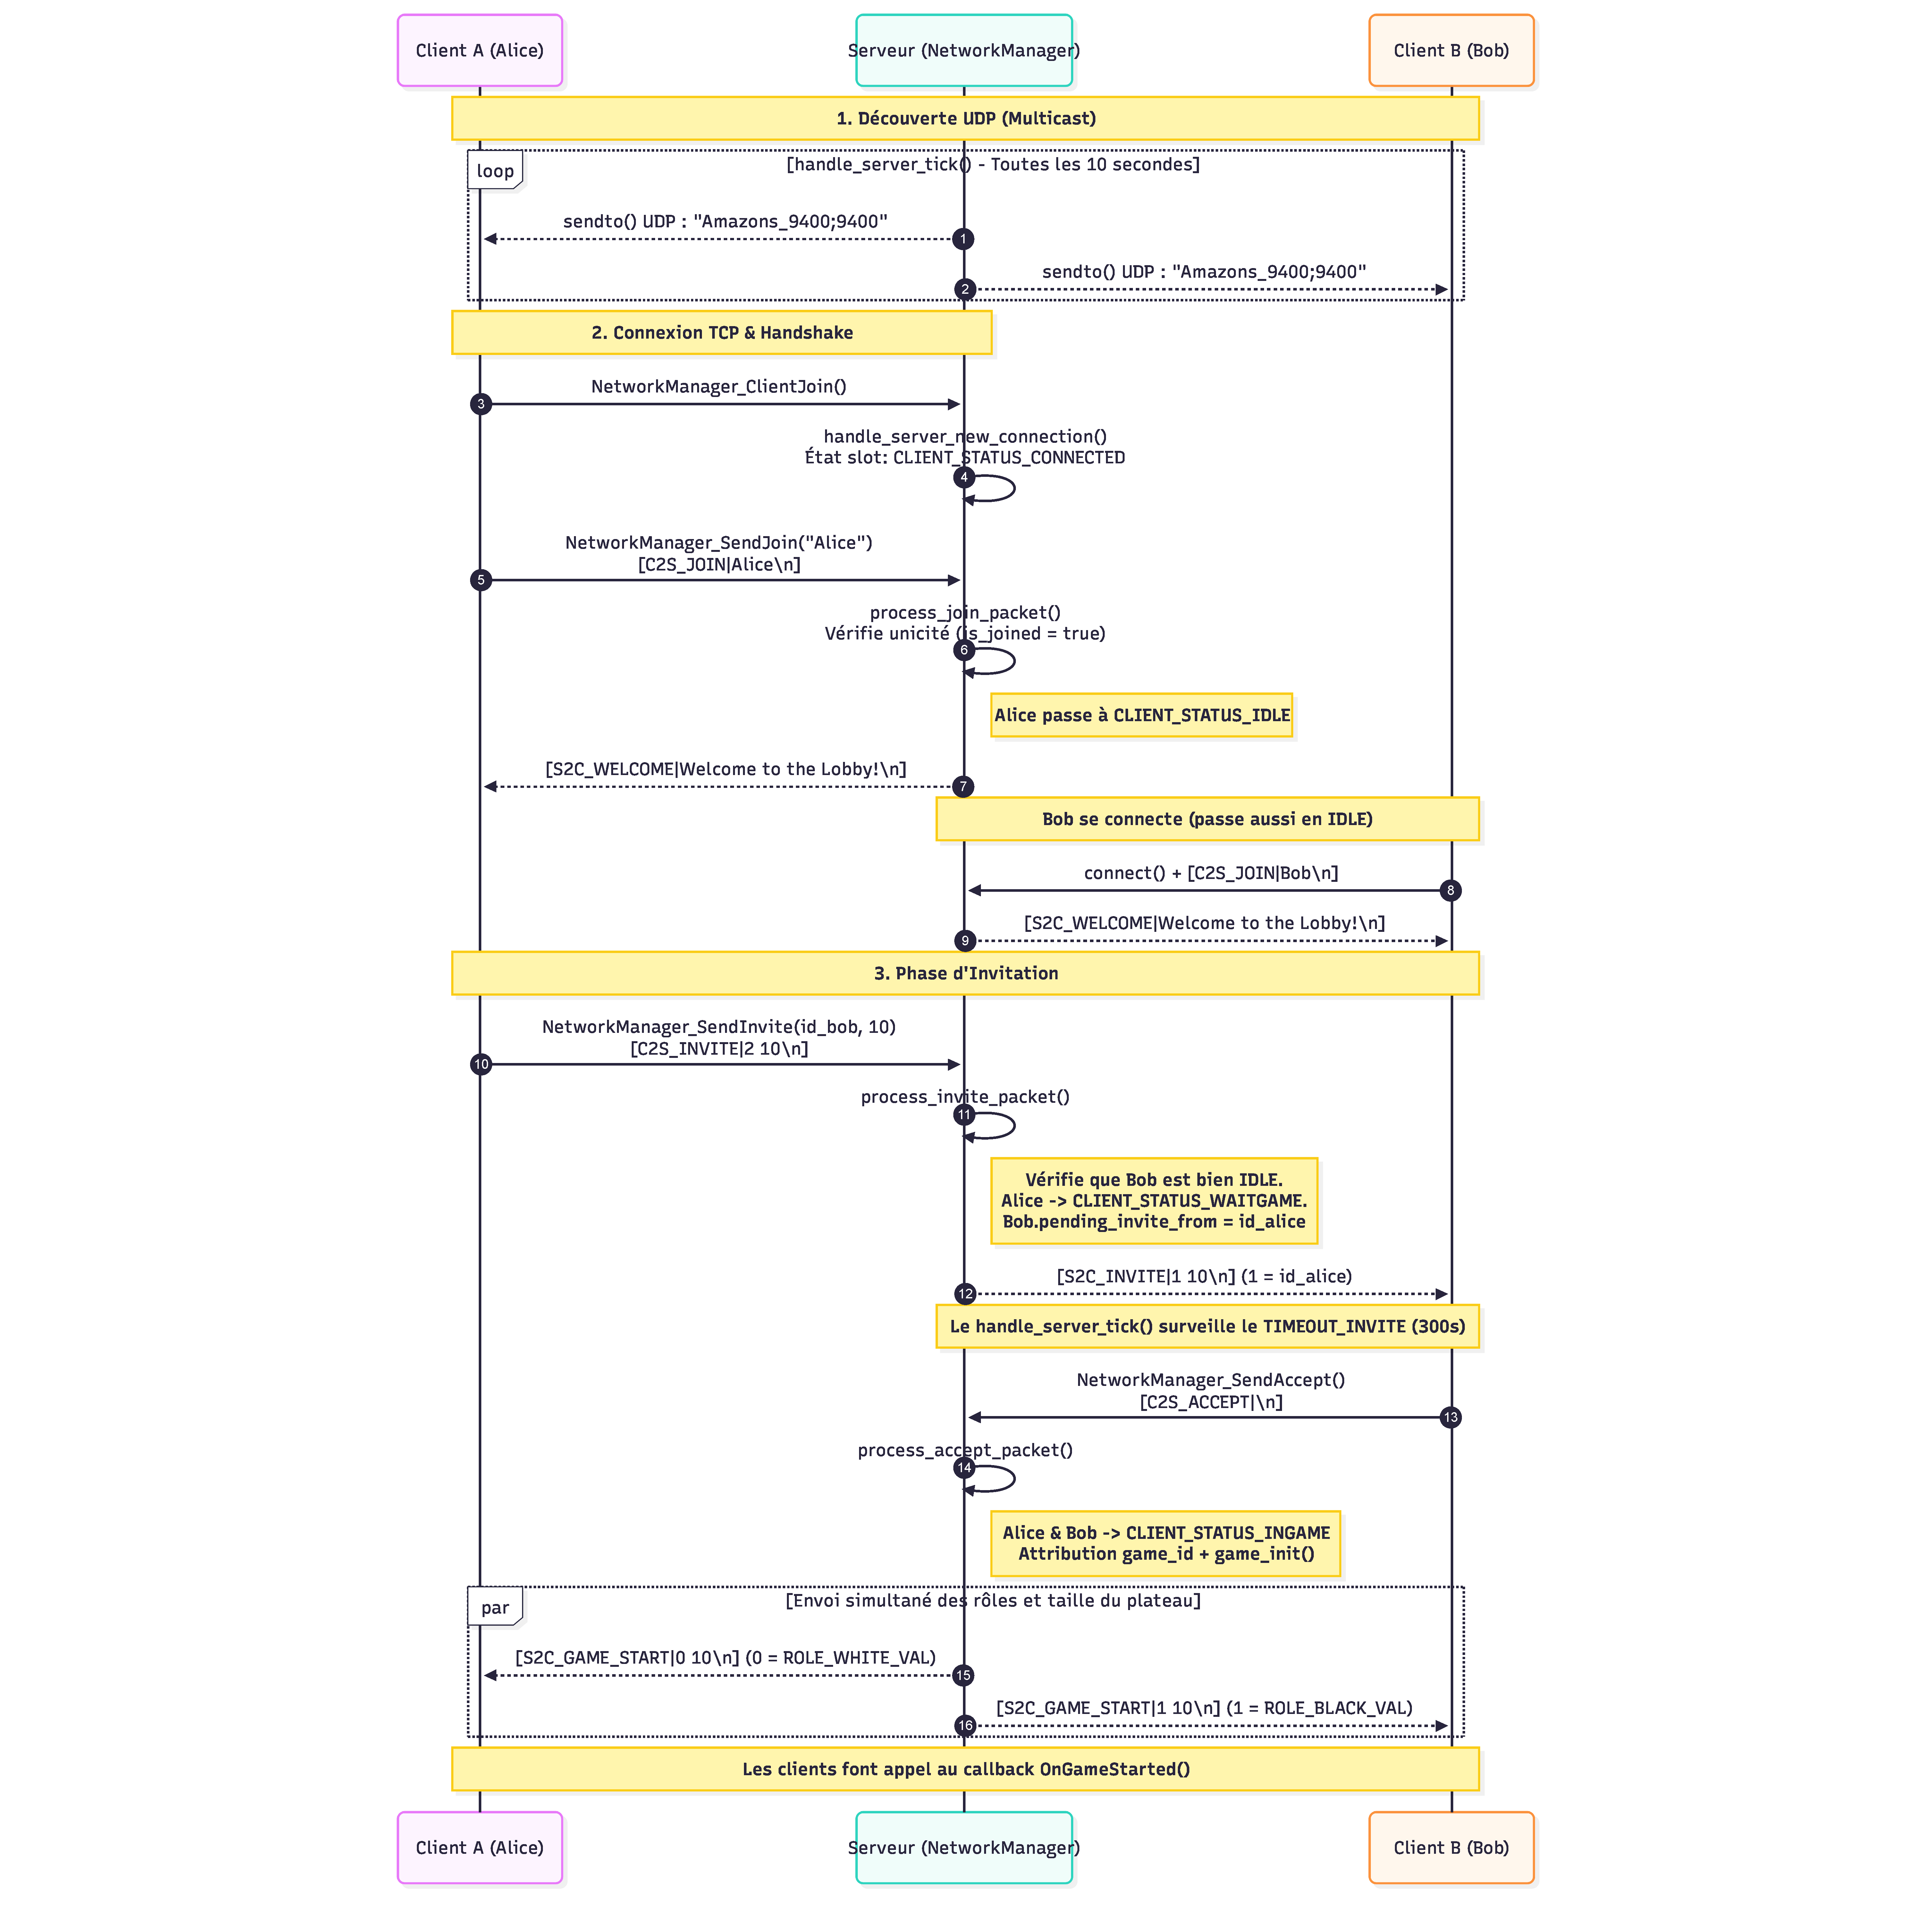
\includegraphics[width=1.35\textwidth]{9400 Alice Flow.pdf}}
    \caption{Protocole d'établissement d'une partie~: découverte UDP, authentification, invitation et démarrage synchronisé.}
    \label{fig:seq_handshake}
\end{figure}


\begin{figure}[H]
    \makebox[\textwidth][c]{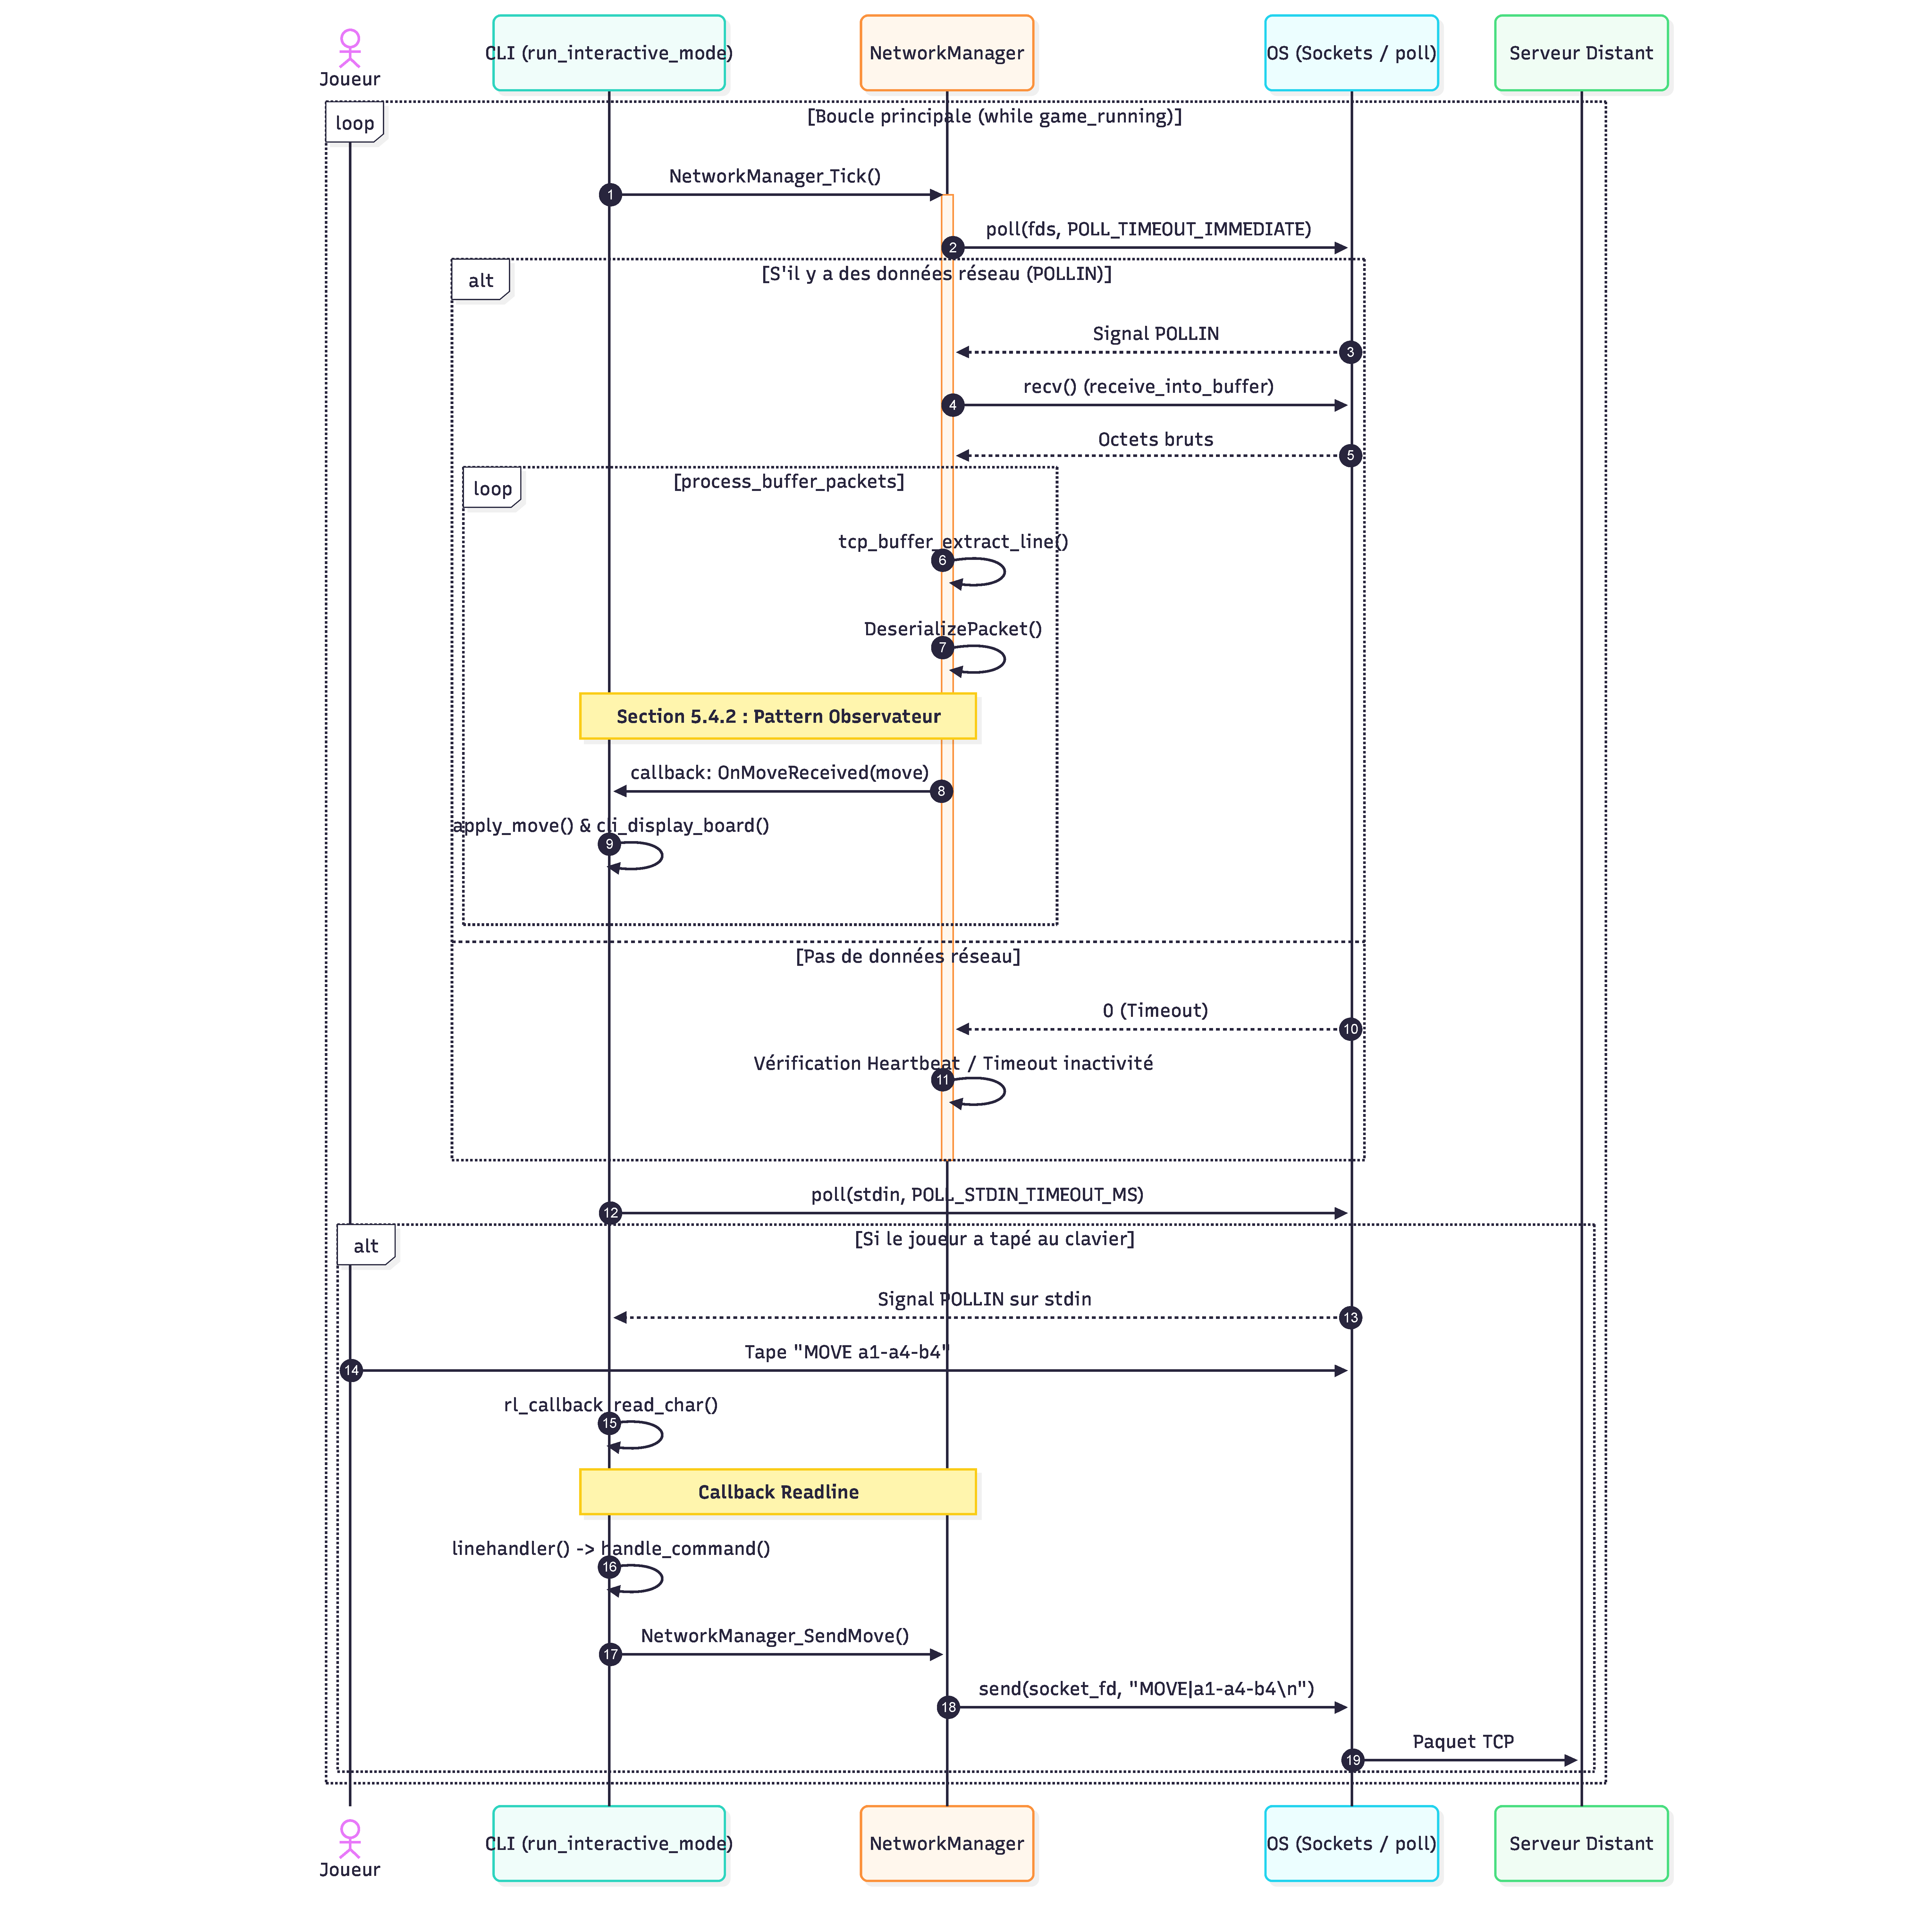
\includegraphics[width=1.35\textwidth]{Interactive Game Network.pdf}}
    \caption{Boucle principale asynchrone~: alternance entre écoute réseau et lecture clavier via deux appels \texttt{poll()} non bloquants.}
    \label{fig:seq_multiplexing}
\end{figure}
\end{document}